\documentclass[11pt]{article}
\usepackage{spikey}
\usepackage{amsmath}
\usepackage{amssymb}
\usepackage{soul}
\usepackage{float}
\usepackage{graphicx}
\usepackage{hyperref}
\usepackage{xcolor}
\usepackage{chngcntr}
\usepackage{mathrsfs}
\usepackage{centernot}
\usepackage[shortlabels]{enumitem}
\usepackage{verbatim}

\usepackage[margin=1truein]{geometry}
\usepackage{setspace}
\linespread{1.15}

\title{Analysis on PANSS Dataset\\ \small STATS 202: Data Mining and Analysis, Final Project}
\author{Tianyu Du}
\date{\today}

\begin{document}
	\maketitle
	\tableofcontents
%	\newpage

	\section{Introduction}
%	\subsection{PANSS Dataset}
	\paragraph{}The Positive and Negative Syndrome Scale (PANSS) score is widely used as a measure for schizophrenia and other disorders in clinical trials. PANSS scores are collected by trained raters and reported by patients or their relatives. One assessment of PANSS scores consists 30 sub-scores from 3 sub-categories: 7 positive scores, 7 negative scores, and 16 general scores. Every score ranges from 1 to 7 denoting increasing levels of psychopathology. The aggregation of all 30 scores provides a detailed assessment of patient's current psychological status.
	
	\paragraph{}The entire dataset consists of five different studies ranging from study A to study E. In this practice, the first four datasets are used as a training to fit, select, and evaluate models. Then, these selected models are used to recover missing data in study E.
	
	\section{Treatment Effects}
	\paragraph{}This section is devoted to analyze whether the treatment assigned leads to significant improvements on patients' psychological status. Because the 18-th week assessments are missing in the dataset of study E, in this section, only data from study A to D are considered. There are 20947 observations (assessments) from above-mentioned dataset, in which 10524 observations came from patients assigned to the control group, and the remaining 10423 were from participants belonged to the treatment group. The evenly-split dataset allows us to deploy various models to analyze whether there exists significant treatment effects.
	
	\paragraph{}Multiple evidences were found to support that there were indeed no treatment effect in this study. Firstly, the effects on four aggregate scores are analyzed, namely sum of all PANSS scores, and sums of scores from positive (\texttt{P\_Total}), negative (\texttt{N\_Total}), and general (\texttt{G\_Total}) sub-categories respectively.
	
	\paragraph{}One challenge associated with treatment effect analysis is the initial status of patients in different groups. In some cases, the \emph{prior} psychological status for a randomly selected patient from the treatment group is expected to be different from that of a random patient in the control group. In these cases, even if significant differences in PANSS scores \emph{posterior} to the treatment were supported, one will not be able to distinguish whether the "effect" came from the discrepancy in the prior distributions or the treatment, and the treatment effect is not well-identifies.
	Figure 1 below presents the distributions of the four aggregate scores at day 0 visit. Both groups shared similar histograms in terms of all four metrics. Moreover, the estimated kernel densities collided, which provided further evidence that there were no significant prior discrepancies between patients from these two groups. Therefore, one can conclude that most posterior differences in PANSS metrics were resulted from the treatment assigned.

	\begin{figure}[H]
		\centering
		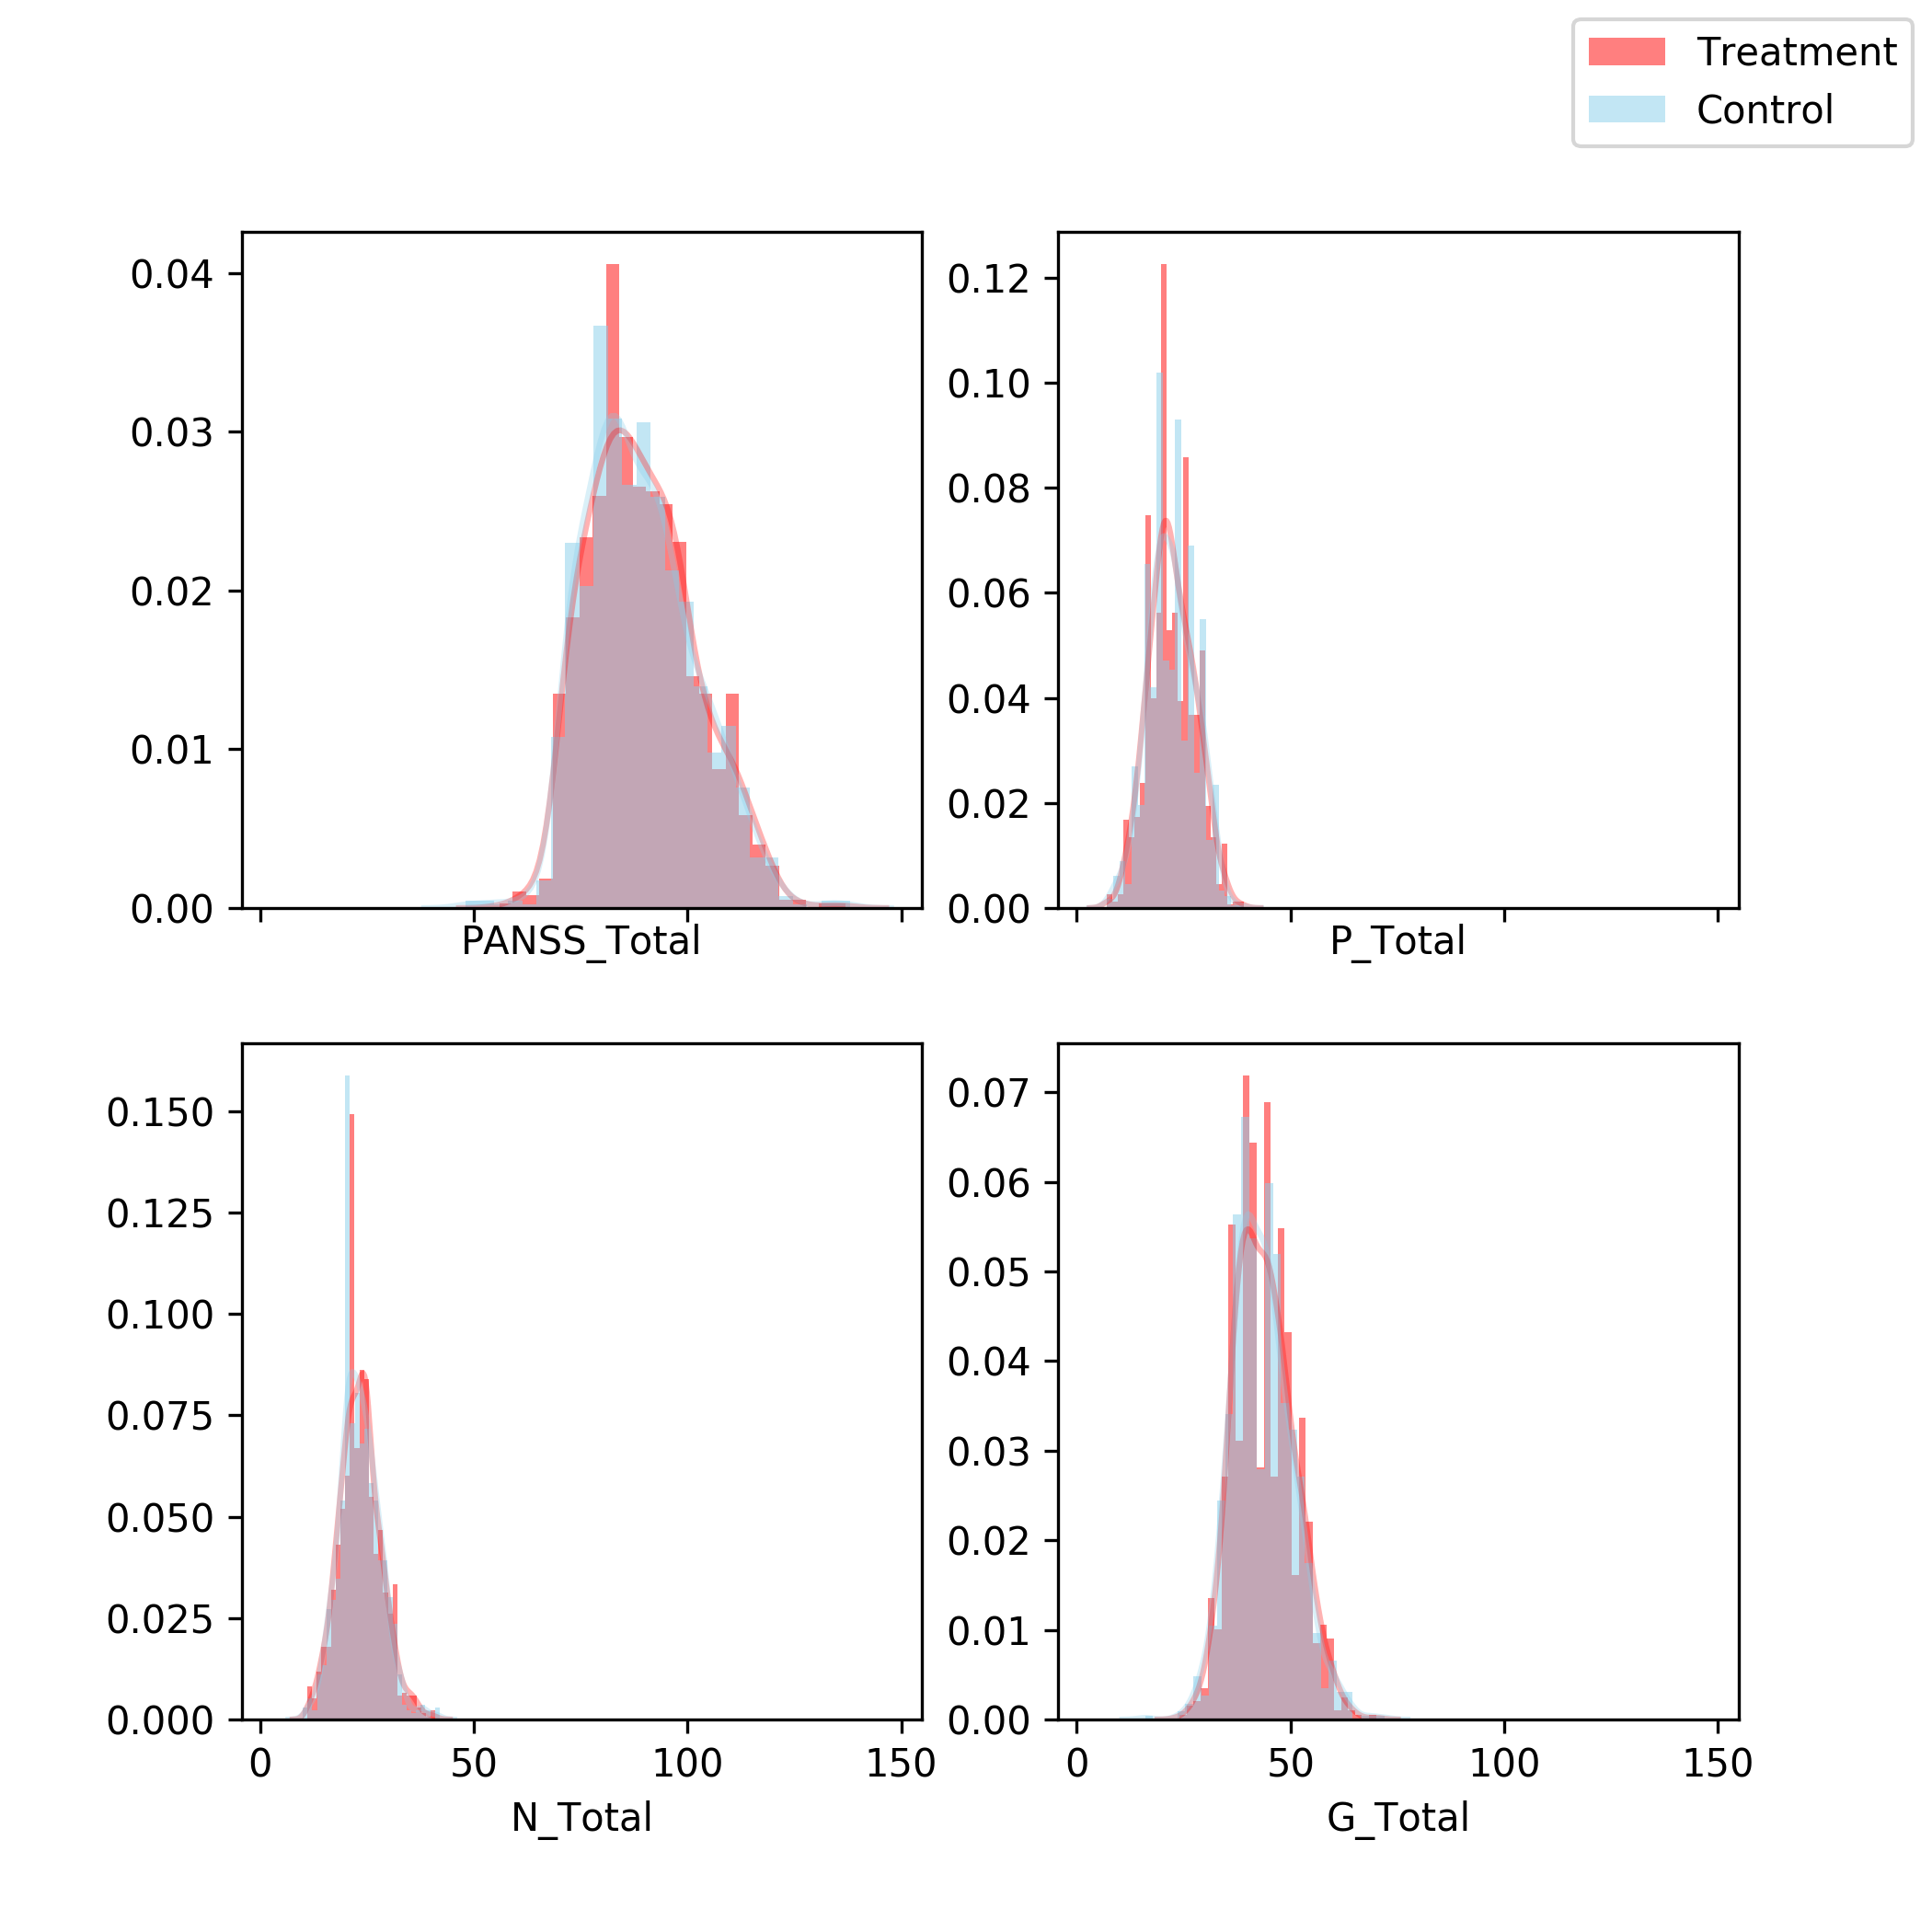
\includegraphics[width=0.7\linewidth]{figures/dist_initial_scores.png}
		\caption{Distributions of Aggregate Scores at Day 0}
	\end{figure}

	\paragraph{}The evolving path of these four above mentioned metrics can provide reasonable proxies to the treatment effect. As mentioned before, we believed the data failed to provide sufficient evidence to support the existence of treatment effect. Let $t \in \N$ denote the \texttt{VisitDay} variable in the dataset, $t$ ranges from 0 to 480 in the complete dataset. Figure 2 presents the distribution of $t$, the 95-percent quantile is located at $t_{95\%} = 297$. Therefore, the top 5\% of observations occupied more than on third of the total range of $t$, these observations are potentially troublesome as outliers. To deal with this issue, the top 5\% observations are excluded from following analysis.

	\begin{figure}[H]
		\centering
		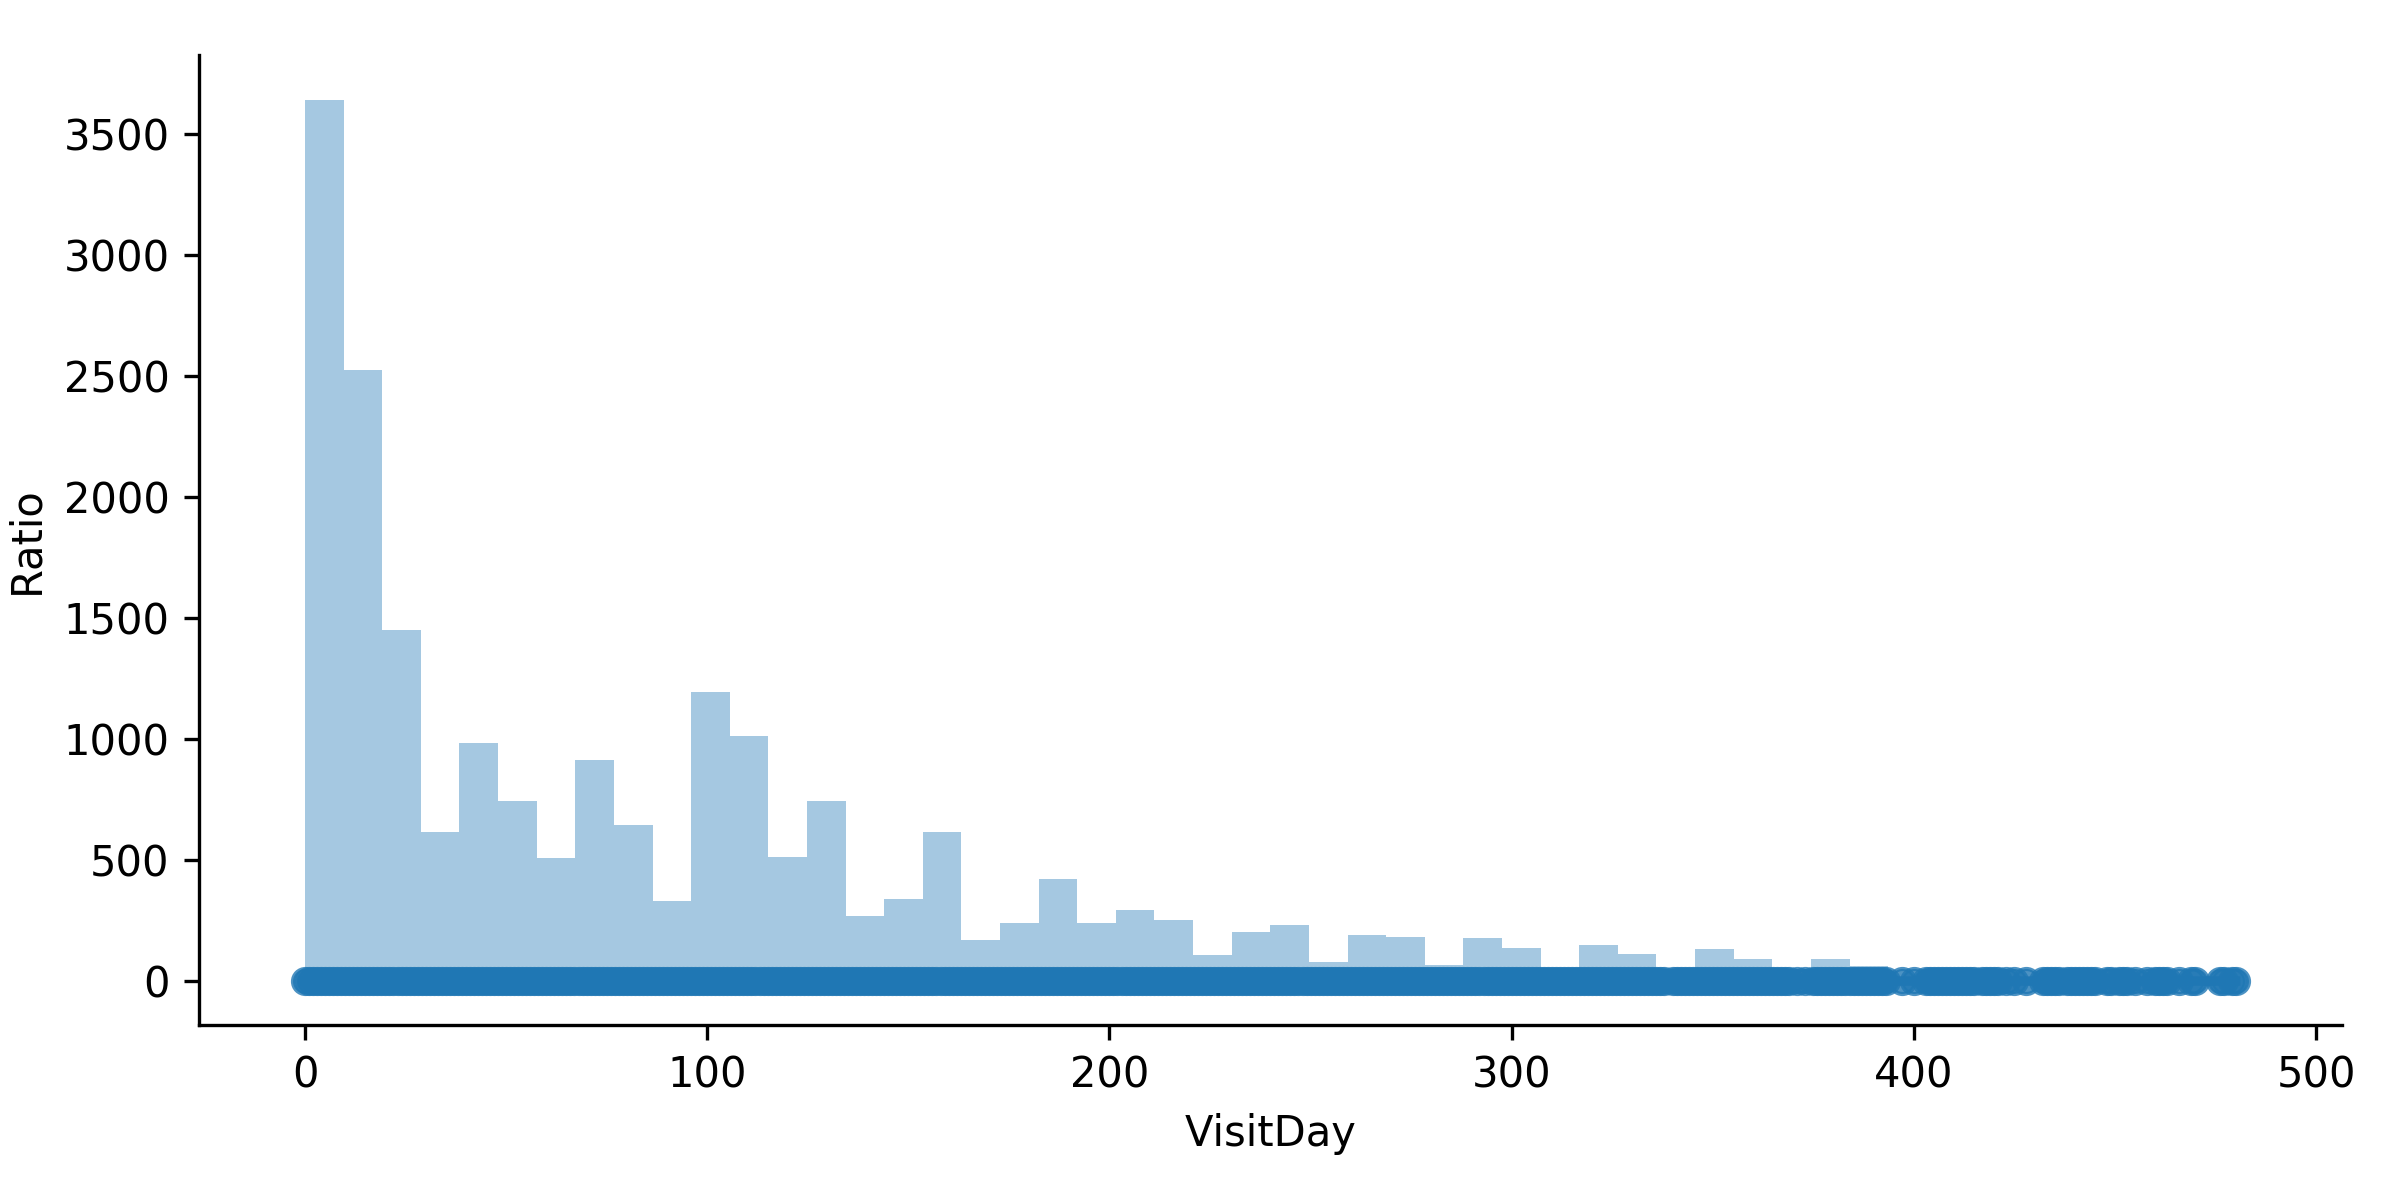
\includegraphics[width=0.7\linewidth]{figures/dist_visit_day_all.png}
		\caption{Distribution of \texttt{VisitDay}}
	\end{figure}
	
	\paragraph{}The general strategy to identify treatment effect here uses linear models. Let $Y$ denote the target metric, which takes value from the four aggregate PANSS metrics: $\mc{M} := \{ \Sigma_{PANSS}, \Sigma_P, \Sigma_N, \Sigma_G\}$. Let $X$ denote the set other characteristics of the patient. And a hybrid linear model is fit:
	\begin{align}
		Y &= f_0(X, t) + \id{\texttt{Treatment}} f_1(X, t)
	\end{align}
	where $f_0$ and $f_1$ are two additive linear models, so that $f_0$ captures the evolving path of $Y$ over time for the population of the control group, and the additive term $f_1$ measures the discrepancy of the treatment group.
	Should the treatment dummy variable is statistically significant, then one can conclude the existence of treatment effect.
	\subsection{Patterns of PANSS over Time}
	\paragraph{}Figure 3 below shows the scatter plot of $\Sigma_{PANSS}$ scores against time for both groups with corresponding locally weighted linear regression estimations (LOWESS). The LOWESS for the treatment and control groups almost collide perfectly, which means the trends for both group estimated from non-parametric model are essentially identical, this provides preliminary evidence supporting our claim that there was no significant treatment effect.
	\begin{figure}[H]
		\centering
		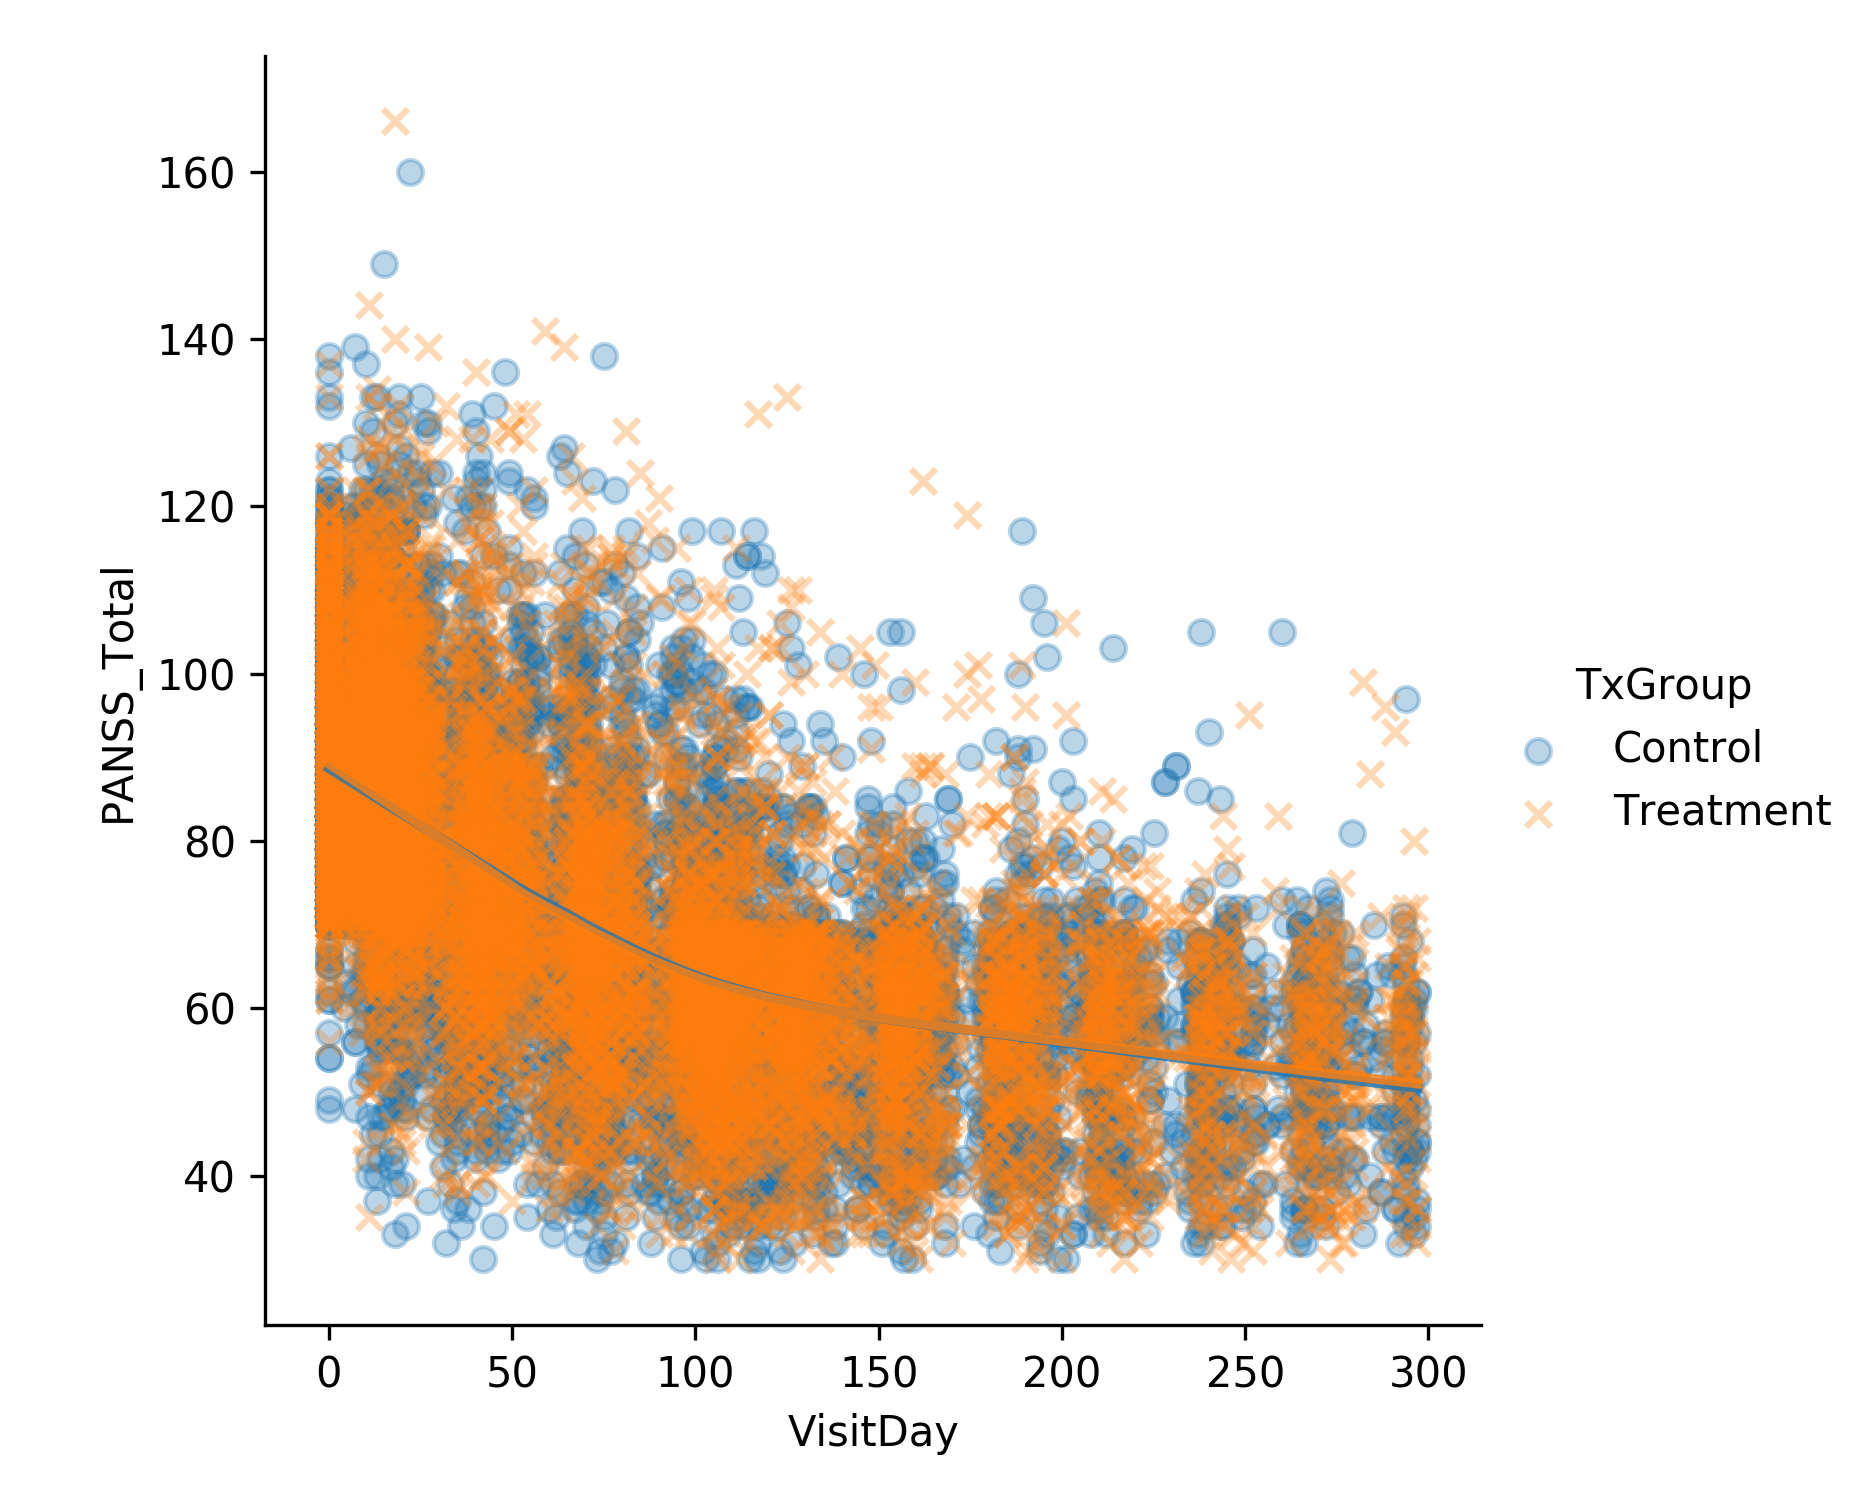
\includegraphics[width=0.7\linewidth]{figures/lwlm_te_PANSS_Total.png}
		\caption{Changes of \texttt{PANSS\_Total} Over Time and LOWESS}
	\end{figure}
	\subsection{Identifying Treatment Effect with Hypothesis Testing}
	\paragraph{} As the plot in figure 3 suggests, the relationship between PANSS scores and $t$ is more or less quadratic. Moreover, similar quadratic characteristics were also found on the other three aggregate metrics (see appendix). Therefore, $f_0$ and $f_1$ are identified as quadratic functions of $t$, specifically,
	\begin{align}
		Y &= f_0(X, t) + \id{\texttt{Treatment}} f_1(X, t) \\
		&= \left(\beta_{0, 0} + \beta_{0, 1} t + \beta_{0, 2} t^2 + \vec{\gamma}_0 \texttt{Country} + \vec{\delta}_0 \texttt{Study}\right) \\
		&+ \id{\texttt{Treatment}} \left(\beta_{1, 0} + \beta_{1, 1} t + \beta_{1, 2} t^2 + \vec{\gamma}_1 \texttt{Country} + \vec{\delta}_1 \texttt{Study}\right) + \varepsilon \\
		&= \theta_0 + \theta_1 t + \theta_2 t^2 + \theta_3 \id{\texttt{Treatment}} + \theta_4 \id{\texttt{Treatment}} t + \theta_5 \id{\texttt{Treatment}} t^2 + \\
		&+\vec{\gamma}_0 \texttt{Country} + \vec{\delta}_0 \texttt{Study} + Z + \varepsilon
	\end{align}
	where $\texttt{Study}$ and $\texttt{Country}$ denote the collection of dummy variables, and $Z$ denotes the set of interaction terms between variables in $X$ and $\id{\texttt{Treatment}}$. It could be controversial whether to include interacting terms between $\id{\texttt{Treatment}}$ and variables other than $t$. As a result, regression results under all combinations of optional covariates are reported in table 1\footnote{Significance codes:  $0 *** 0.001 ** 0.01 * 0.05 \dagger 0.1 \quad 1$}, in which \texttt{S}, \texttt{C}, and \texttt{T} stand for \texttt{Study}, \texttt{Country}, and \texttt{Treatment} respectively. The negative coefficients of $\texttt{T} \times t$ in different settings suggest the treatment actually helped reduce the severity of schizophrenia. However, due to the large standard error of estimator, almost all of these coefficients were found insignificant. Even though in some rare cases, the treatment indicator on the intercept term were different from zero significantly. Consequently, we conclude that the treatment did no affect how PANSS metrics changed over time, so there are no treatment effect.
	\begin{table}[H]
	\centering
	\begin{tabular}{l|c|c|c|c}
		Covariates from $Z$ & $\varnothing$ & \texttt{C}*\texttt{T} & \texttt{S}*\texttt{T} & \texttt{C}*\texttt{T} + \texttt{S}*\texttt{T}\\
		\hline
		\texttt{PANSS\_Total} $\sim$ \texttt{T}& $0.5167(0.1873)^{**}$& -2.113(1.577)& -0.4924(0.5505) & -3.717(1.798)$^*$ \\
		\texttt{PANSS\_Total} $\sim$ $\texttt{T} \times t$ & -35.95(26.40)& -31.33(26.91)& -36.58(27.18)& -2.811(2.736)\\
		\texttt{PANSS\_Total} $\sim$ $\texttt{T} \times t^2$ & 24.99 (26.36) & 23.72(26.36)& 32.84(26.40)& 2.819(2.641)\\
		\hline 
		\texttt{P\_Total} $\sim$ \texttt{T}& 0.06806(0.06473)& -1.296(0.5447)$^*$ & -0.6036(0.1902) & -2.294(0.6210)$^{***}$\\
		\texttt{P\_Total} $\sim$ $\texttt{T} \times t$ & -7.643(9.121) & -8.135(9.297)& -12.59(9.391)$^{**}$ & -10.58(9.453)\\
		\texttt{P\_Total} $\sim$ $\texttt{T} \times t^2$ & 14.65(9.107)& 1.449(9.108)& 17.65(9.122)$^\dagger$& 14.89(9.126)\\
		\hline
		\texttt{N\_Total} $\sim$ \texttt{T}& 0.1132(0.06793)$^\dagger$& -0.1981(0.5700) & -0.002971(0.1996)& -0.3724(0.6498)\\
		\texttt{N\_Total} $\sim$ $\texttt{T} \times t$ & -10.22(9.571)& -6.610(9.728) & -6.791(9.856) & -2.909(9.890)\\
		\texttt{N\_Total} $\sim$ $\texttt{T} \times t^2$ & 0.4369(9.557)& 1.472(9.530) & 3.389(9.573)& 4.399(9.548)\\
		\hline
		\texttt{G\_Total} $\sim$ \texttt{T}& 0.3353(0.09998)$^{***}$&  -0.6194(0.8418) &  0.1142(0.2939) & -1.051(0.9601)\\
		\texttt{G\_Total} $\sim$ $\texttt{T} \times t$ & -18.09(14.09) & -16.49(14.37)& -17.20(14.51)& -14.62(14.61)\\
		\texttt{G\_Total} $\sim$ $\texttt{T} \times t^2$ & 9.901 (14.07)& 7.751(14.08) & 11.80(14.10)& 8.900(14.12)\\
	\end{tabular}
	\caption{Regression Results with Different Combination of Variables (Standard Error in Parenthesis)}
	\end{table}

	
	\section{Patient Segmentation}
	\paragraph{} In this section, segmentation methods were deployed to cluster 2438 patients based on their PANSS metrics at day zero. Two decisions must be made during this process: (i) how many clusters to use(ii); and what type of cluster to use.
	\subsection{Preprocessing}
	\paragraph{} Even though the prior ranges of all PANSS sub-scores were the same, they had different sample variance. Most clustering algorithms are sensitive to the mean and variance of features. To avoid potential issues, all 30 sub-scores were standardized before applying clustering on them.

	\subsection{Identify Optimal Number of Clusters}
	\paragraph{} Elbow method can provide us song rough idea on the number of clusters to use. By analyzing the improvement in total (within group) sum of squares from adding more clusters, one can observe that adding one more cluster after $k=7$ did not provide much improvement. We can conclude that the optimal $k$ would lie between 2 and 7.
	
	\begin{figure}[H]
		\centering
		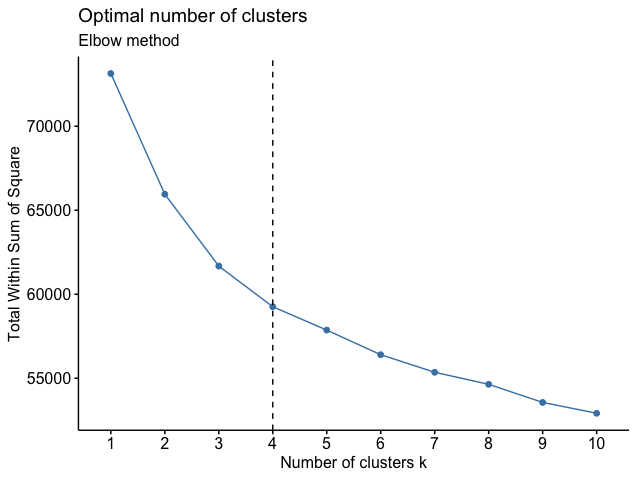
\includegraphics[width=0.7\linewidth]{figures/Elbow_method.png}
		\caption{Elbow Method to Identify Number of Clusters}
	\end{figure}
	
	\paragraph{} To find the optimal value of $k$, we used \texttt{NbClust} package in \texttt{R}, which implemented 30 criterions to identify the optimal $k$. Each criterion proposed one optimal $k$, and the final number of clusters was set to be the one proposed by most criterions. According to the result, three was the number of clusters supported by most criterions (by 14 criterions).

	\subsection{Choosing Clustering Algorithms}
	\paragraph{} Agglomerative algorithms with four different types of linkages were deployed together with k-means. As mentioned above, the optimal number of clusters was identified to be three. The experiment implied k-means delivered a more balanced segmentation in terms of group sizes when $k=3$. As a result, k-means with three clusters were used in following sections.
	
	\begin{table}[H]
		\centering
		\begin{tabular}{l|c|c|c}
			Model & 2 Clusters & 3 Clusters & 4 Clusters \\
			\hline
			\hline
			Agglomerative \\
			\hline
			Ward & (1714, 724) & (1714, 452, 272) & (860, 854, 452, 272) \\
			Complete & (2178, 260) & (2177, 260, 1) & (1580, 597, 260, 1) \\
			Average & (2437, 1) & (2436, 1, 1) & (2435, 1, 1, 1) \\
			Single & (2437, 1) & (2436, 1, 1) & (2435, 1, 1, 1) \\
			\hline
			\hline
			K-Means & (1411, 1027) & (882, 828, 728) & (787, 642, 543, 466)
		\end{tabular}
		\caption{Group Sizes from Different Algorithms}
	\end{table}
	
	\subsection{Visualization and Evaluation}
	\paragraph{} Ideally, one create a scatter plot of observations, and then mark instances belonging to different clusters using different colours, and tell whether the clustering algorithm provides reasonable segmentation. However, it is impossible for us to visualize feature space beyond three dimensions.\footnote{Theoretically, one can draw the fourth dimension by colouring observations differently. But in our case, colours are used to identify clusters.} Instead, clustering results were plotted using reduced feature spaces. PANSS sub-scores were inherently defined using three sub-groups, it is natural to use the summations of sub-scores belongs positive, negative, and general scores as three axes of the reduced feature space.
	\paragraph{} In additional, the reduced feature space of the first three principle components was used as well. Since the clustering algorithm only had access to standardized scores but not principle components, a clustering algorithm is dong a good job if the clustering result provided also segment the principle component space reasonably as well. Figures below present the clustering result on both reduced feature spaces mentioned above. From the plot on PANSS scores, one can observed that the green group was featured by high scores in all three aggregate metrics, which is likely corresponding to the high-severity patients.	While the orange group was characterized by low positive score with moderate negative and general scores. This group could be low-severity patients. Members in the blue group in general had above average positive scores, average general score, and low negative scores.\footnote{Statements here might be hard to observe using the static 3D plot, one can either run the script to generate an interactive 3D plot or check corresponding 2D plots in appendix.}
	\begin{figure}[H]
		\centering
		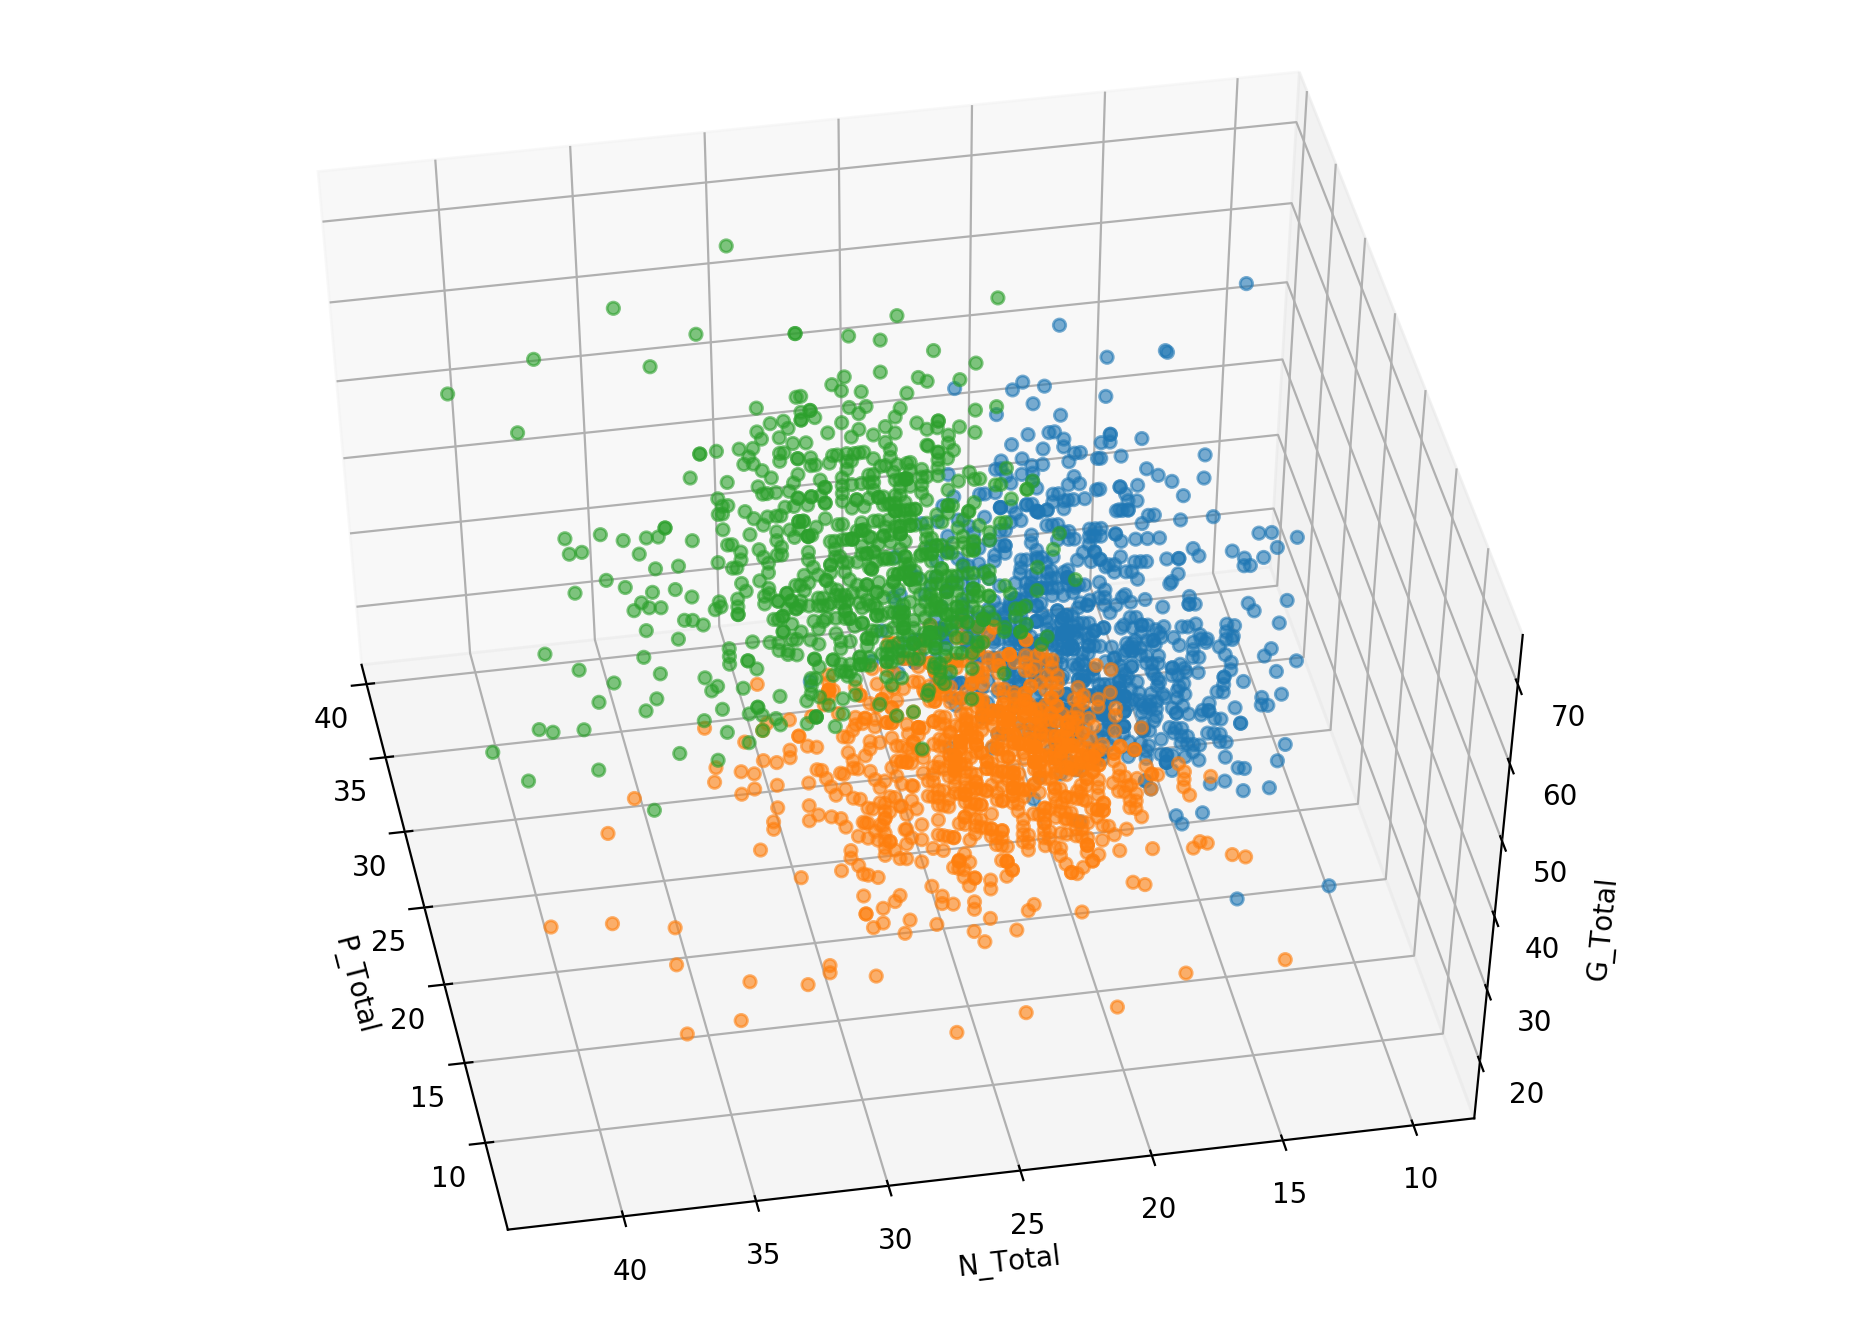
\includegraphics[width=0.7\linewidth]{figures/kmean_3.png}
		\caption{K-Mean Result On Aggregate Metrics of PANSS}
	\end{figure}
	Moreover, k-mean clustering result seemed to stay valid on the principle component space, which further fortify the algorithm chosen.
	\begin{figure}[H]
		\centering
		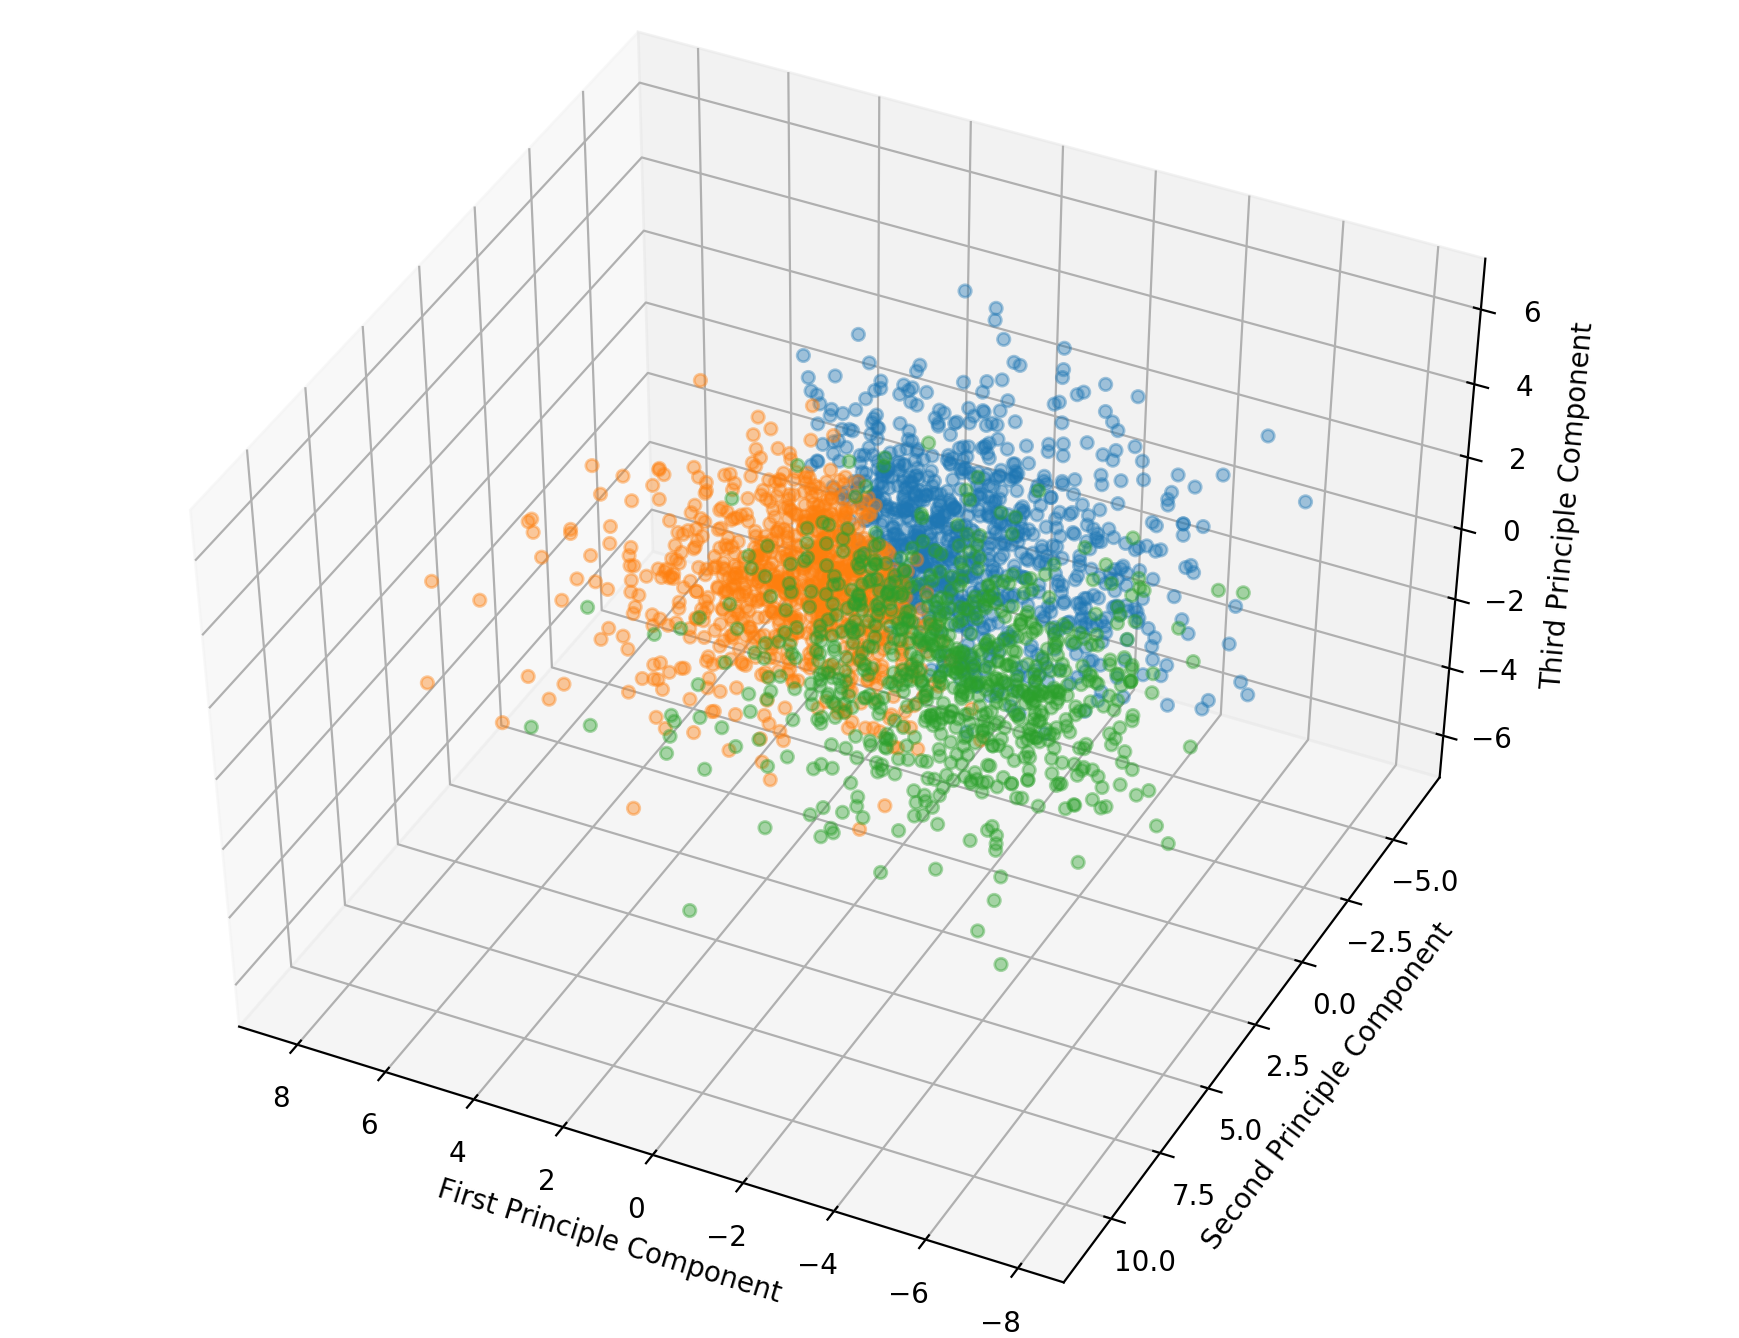
\includegraphics[width=0.7\linewidth]{figures/k_mean_on_pca.png}
		\caption{K-Mean Result on Principle Components}
	\end{figure}
	
	\section{Patient 18-th Week PANSS Forecasting}
	\subsection{Feature Space}
	\paragraph{} This section is devoted to forecasting the total PANSS scores in the last visit of each participating patient. Several variables including indicator for treatment and country were invariant throughout the experiment period. The binary \texttt{TxGroup} variable was simply reduced to one binary variable \texttt{Treatment} $:= \id{\texttt{TxGroup} = \tx{Treatment}}$.
	
	\paragraph{} There are 284 unique site IDs and 639 unique rater IDs. Because IDs are numerical but not ordinal values, adding these two features would require an addition of more than 900 one-hot variable, which is significantly larger than the number of raw PANSS scores. Including them could be helpful, but at a risk of potential overfitting and cruise of dimensionality. Therefore, these IDs were excluded.
	\paragraph{} Assessments in the dataset came from 27 different countries (figure below). Note that there are 18 assessments (belong to 3 patients) do not possess valid values for country. To reduce the dimension of feature space, and handle issue when there are incoming patients from countries not in the training set (there were patients from UK in the test set, but not in the training set), only information on the top five countries was preserved, and all other countries were reduced to one single "other" category. As a result, the \texttt{Country} feature in the raw dataset was transformed into six one-hot-encoded dummies: \texttt{Country\_USA}, \texttt{Country\_Ukraine}, \texttt{Country\_Japan}, \texttt{Country\_Russia}, \texttt{Country\_China}, and \texttt{Country\_Other}.
	\begin{figure}[H]
		\centering
		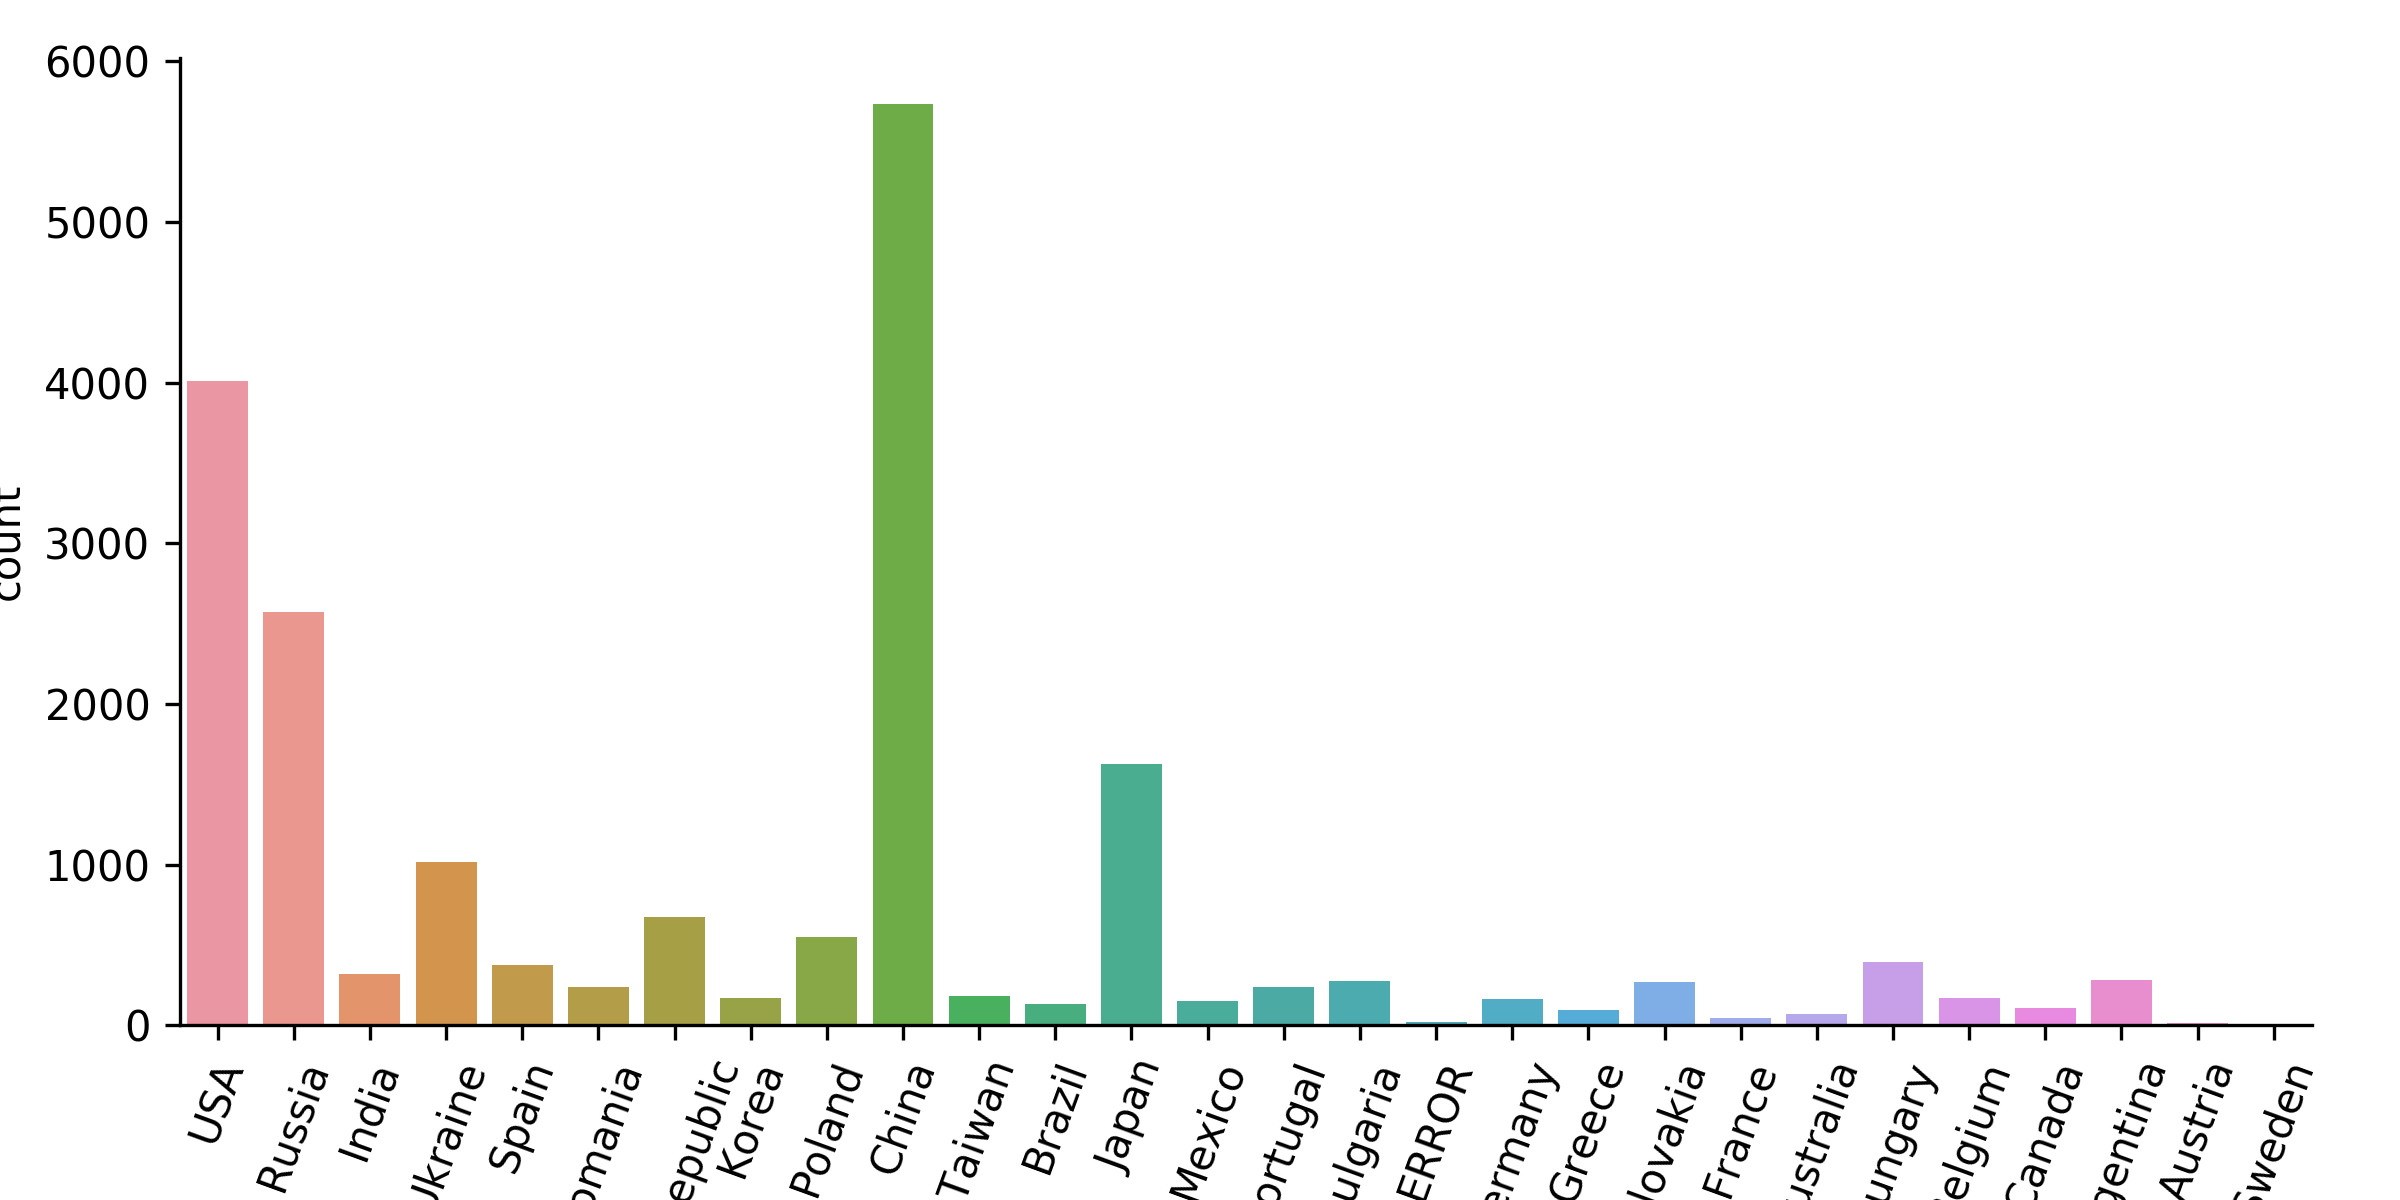
\includegraphics[width=0.7\linewidth]{figures/dist_country.png}
		\caption{Distribution of \texttt{Country}}
	\end{figure}
	
	\paragraph{} Each of the 1826 patients in the training set had different numbers of visits on record, most statistical learning models admit dataset in which all training instances have the same number of features. To accommodate this, summary statistics of PANSS scores instead of all scores were used together with time-invariant features like country and treatment. Specifically, the mean, maximum, minimum, and standard deviations of each PANSS sub-score were included. In additional, scores at day 0 and the last visit before the 18-th week visit were used as well to better capture patient's psychological status.

	\subsection{Ensemble Method: Random Forest}
	\paragraph{} Even though not all PANSS records were fed to the model, there were still hundreds of features actually used. To prevent risks from overfitting, a random forest model is proposed. The grid searching suggested that an ensemble of 500 deep trees with depth of 4096 preformed best in terms of MSE estimated using 5-fold cross validation.

	\subsection{Support Vector Regression with Polynomial and RBF Kernel}
	\paragraph{} Support vector regressions use different kernels to engineer input features implicitly. Two commonly chosen kernels are polynomial and RBF kernels. SVRs in general take longer to fit than other methods, but deliver superior performances. The scopes of hyper-parameter searching for different kernels are presented in tables below.
	\begin{table}[H]
		\centering
		\begin{tabular}{l|c|c|c}
 		H-Param & Range & Best & Total \\
 		\hline
 		\hline
 		Polynomial Kernel \\
 		\hline
 		Kernel Size ($\gamma$) & $\{\frac{1}{p}, 0.1, 0.01, 0.001, 0.0001\}$ & 0.0001 & 5 \\
 		Err. Penalty ($C$)& $\{2, 4, 8, 16\}$ & 4 & 4 \\
 		Polynomial Deg. ($\delta$)& $\{3, 4, 5, 6\}$ & 3 & 4 \\
 		\hline
 		All Combinations & & & 80 \\
 		\hline
 		\hline
 		RBF Kernel \\
 		\hline
 		Kernel Size ($\gamma$) & $\{\frac{1}{p}, 10^{-10}, 10^{-9}, \cdots 0.1\}$ & $10^{-5}$ & 10 \\
 		Err. Penalty ($C$)& $\{2, 4, 8, \cdots, 516\}$ & 128 & 9 \\
 		\hline
 		All Combinations & & & 90
		\end{tabular}
		\caption{Hyper-parameter Scope and Result for Support Vector Regression}
	\end{table}

	\subsection{Ensemble Method: Gradient Boosting}
	\paragraph{} Gradient boosting machines refine predictions by iteratively fitting additional models on the residual from previous models.
	
	\subsection{Summary on Model Performance}

	\section{Assessment Validity Classification}
	\subsection{Feature Space}
	\paragraph{} In this section, each assessment becomes one training instance. The feature space consists of 30 PANSS scores and several identifiers such as country and rater's ID. In this study, all 30 PANSS scores and \texttt{PANSS\_Total} were taken to be preliminary features. As for treatment and country identifiers, the same procedure mentioned in the previous section was followed.
	\paragraph{} In the training set, the standard deviations of 30 PANSS sub-scores range from 0.9374 to 1.562, and their averages range from 1.572 to 3.258. To eliminate this discrepancy, These 30 metrics were standardized so that all of them share mean of zero and standard deviation of one.
	\paragraph{} Moreover, the figure below plots out the fraction for an assessment taken on particular visiting day to be flagged or assigned to CS. The plot suggests a nontrivial relation between the empirical probability of anomaly assessment and the day of visit. Therefore, \texttt{VisitDay} is also included as a feature.
	\begin{figure}[H]
		\centering
		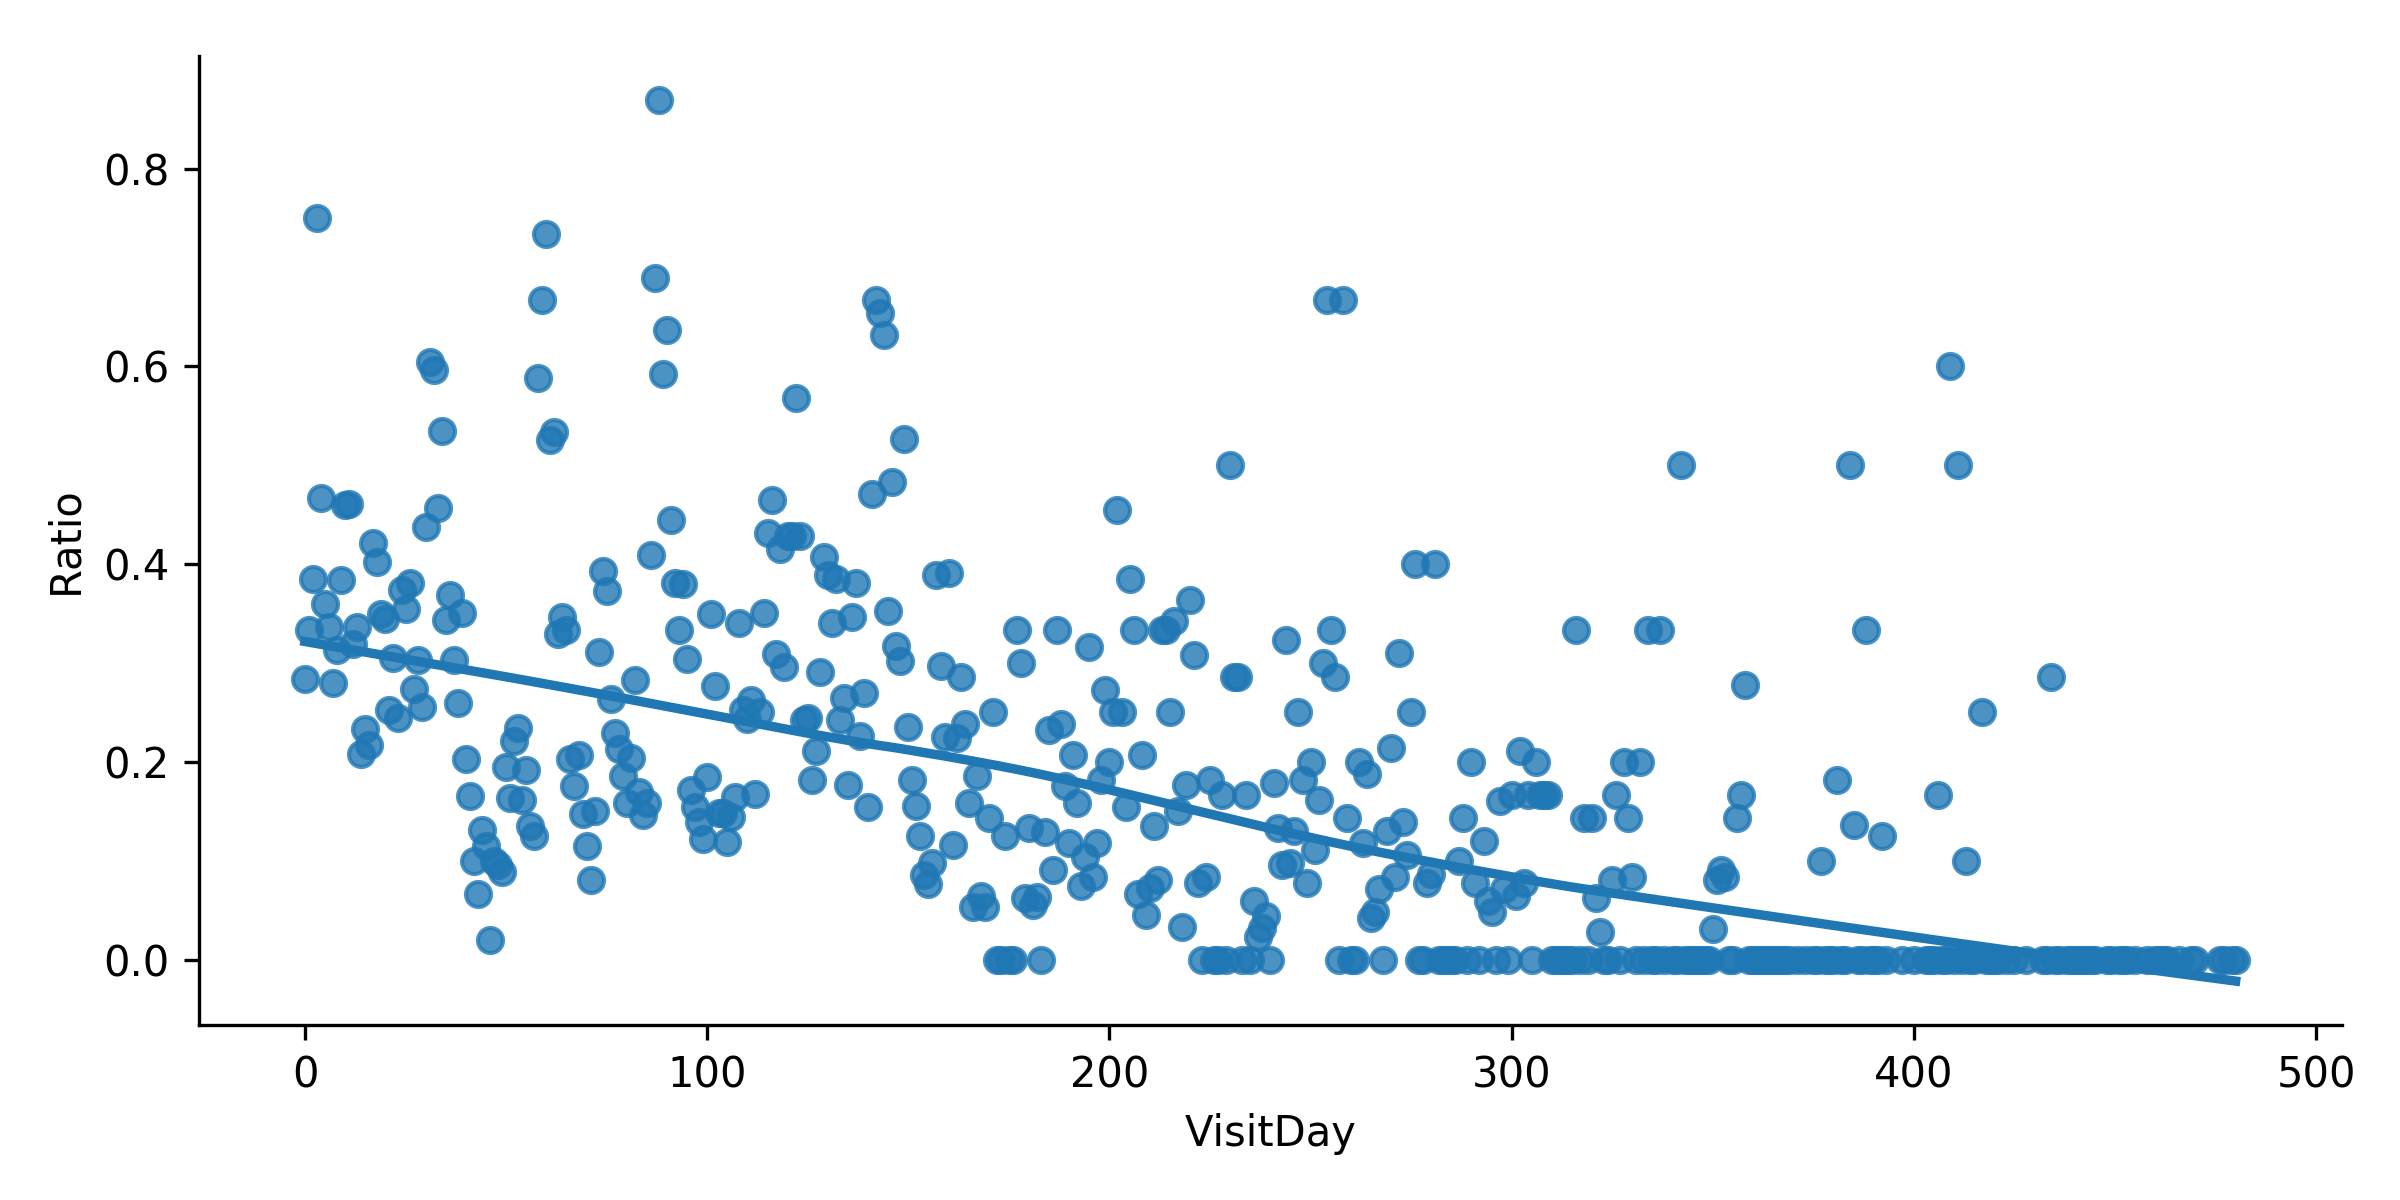
\includegraphics[width=0.7\linewidth]{figures/alert_ratio_days.png}
		\caption{Fraction of Assessments Flagged on Each Day}
	\end{figure}
	
	\subsection{General Strategy to Identify the Best Learner}
	\paragraph{} In the following parts of this section, various models are proposed for the classification task using features mentioned before.
	\paragraph{} In general, the hyper-parameters of each model must be tuned over a large hyper-parameter space $\mc{M}$. However, it is infeasible to search over the entire hyper-parameter space as there are uncountably infinite combination of hyper-parameters for each model. Instead, a grid search algorithm with cross-validation was deployed. Firstly, a finite subset of $\mc{M}$, $\mc{G}$, was constructed manually, in which each element $g \in \mc{G}$ characterizes a valid model. Then for each $g \in \mc{G}$, the grid search algorithm fit a model with hyper-parameter set $g$ five times on different training sets given by a 5-fold cross validation.
	\footnote{Due to the time constraint, 5-fold CV was used instead of the more conventional 10-fold CV. Typically, hundreds of possible configurations were searched over for each type of model, using $k$-fold CV requires $k \times |\mc{G}|$ model fitting. While $k=5$, the grid search for each type of model took around 4 hours on a 64-core server, it seemed to be infeasible to run grid search with $k=10$.}
	And the generalization error for such model is estimated using the collection of different CV test sets. Then, for each category of models (random forest, neural nets, etc), the hyper-parameter set  achieved the best CV performance measured by cross-entropy loss was saved to represent the best performance for this model category.
	
	 \paragraph{} After the best hyper-parameter set for each type of learner was identify, they were evaluated again using $k$-fold cross validation techniques to make comparisons across different types of models, where $k$ depends on the actual time taken to train particular model.
	
	\subsection{Baseline Model: Logistic Regression}
	\paragraph{} A logistic regression model is used as a performance baseline. There are only few customization can be made on logistic regression, the grid search looked over the inverse of regularization strength $C$ and the form of regularization. An elastic net regularization was applied to the baseline logistic regression and the regularization takes form $\alpha \norm{\theta}_1 + (1 - \alpha) \norm{\theta}_2$, where $\alpha \in [0, 1]$ controls the exact form of regularization term. The grid search results suggested a logistic regression with almost fully L-1 regularization performed the best.
	\begin{table}[H]
		\centering
		\begin{tabular}{l|c|c|c}
		H-Param & Range & Best & Total \\
 		\hline
 		Inverse Reg. ($C$) & $\{2^{-10}, 2^{-9}, \cdots, 2^9\}$ & $2^{-8}$ & 20 \\
 		L1 Reg. Weight ($\alpha$) & $\{0, 0.2, 0.4, \cdots, 0.98, 1\}$ & 0.98 & 51 \\
 		\hline
 		All Combinations & & & 1020 
		\end{tabular}
		\caption{Hyper-parameter Scope and Result for Logistic Regression}
	\end{table}
 	
 	\subsection{Ensemble Model: Random Forest}
 	\paragraph{} Random forests handles overfitting problems naturally as an ensemble method. Several hyper-parameters play crucial rules while fitting a random forest, including number of tree built, the criterion for choosing the best split, the number of features to consider while identifying the best split, as well as the maximum depth of each tree. Let $\mc{G}$ and $p$ denote the proposed hyper-parameter space and number of features respectively. The table below shows the scope of above mentioned hyper-parameters searched over during the grid search process.
 	\begin{table}[H]
 		\centering
 		\begin{tabular}{l|c|c|c}
 		H-Param & Range & Best & Total \\
 		\hline
 		Max Depth ($\delta$) & $\{\infty, 2, 4, \cdots, 1024\}$ & 64 & 7 \\
 		Num Trees ($\tau$) & $\{100, 300, 500, \cdots, 1900\}$ & 1900 & 10 \\
 		Criterion & Entropy, Gini Coef. & Gini Coef. & 2 \\
 		Max Features ($\phi$) & $\log_2(p), \sqrt{p}$ & $\log_2(p)$ & 2\\
 		\hline 
 		All Combinations& & & 280
		\end{tabular}
		\caption{Hyper-parameter Scope and Result for Random Forest}
 	\end{table}
 	As mentioned before, all 280 candidates were evaluated using 5-CV and cross entropy loss. The best combination of hyper-parameters found after 1400 model fittings was included in the table. Note that the optimal value of $\tau$ was found on the boundary of $\mc{G}$, it is reasonable to suspect that further increase of $\tau$ could lead to an even further improvement in model performance. To accommodate this issue, two additional models with $\tau=2000, 2100$ were evaluated using 5-CV and compared with the best model identified using grid search. It turned out that the improvements in generalization error were both only around $0.4\%$, and the performance even dropped when $\tau$ was risen from $2000$ to $2100$. Therefore, the model identified from grid searching was chosen to represent random forest class.
 	
 	\begin{table}[H]
	 	\centering
		\begin{tabular}{l|c}
			$\tau$ & Avg. Test Err. ($\pm \frac{1}{2}$ Range) \\
			\hline
			1900 & $0.3709(\pm 0.008014)$ \\
			2000 & $0.3693(\pm 0.005638)$ \\
			2100 & $0.3694(\pm 0.01037)$ 
		\end{tabular}
		\caption{Further Increments of Number of Estimators}
	\end{table}
 
 	\subsection{Ensemble Model: Gradient Boosting}
 	\paragraph{} Gradient boosting is another type of ensemble models, in contrast to the parallel ensemble strategy of random forests, GBs ensemble multiple models vertically. For GBs, Friedman mean squared error was used to measure the quality of splits in the boosting process. The table below presents the scope of grid searching and the best combination of hyper parameters identified among all 480 candidates. Note that the optimal values were all in the interior of our pre-defined scope $\mc{G}$.
 	\begin{table}
 		\centering
 		\begin{tabular}{l|c|c|c}
 		H-Param & Range & Best & Total \\
 		\hline
 		Max Depth ($\theta$) & $\{3, 6, 9, 12\}$ & 6 & 4 \\
 		Learning Rate ($\alpha$) & $\{0.001, 0.003, 0.01, 0.03, 0.1, 0.3\}$ & 0.003 & 6 \\
 		Num Estimators ($\tau$) & $\{100, 300, \cdots, 1900\}$ & 700 & 10 \\
 		Max Features ($\phi$) & $\log_2(p), \sqrt{p}$& $\sqrt{p}$ & 2\\
 		\hline
 		All Combinations & & & 480
 		\end{tabular}
 		\caption{Hyper-parameter Scope and Result for Gradient Boosting Machines}
 	\end{table}
 	
 	\subsection{Support Vector Classifier}
 	\paragraph{} Gradient boosting machines used the entire raw feature space and recursively fit new model on the residual of previous model, then ensemble all hierarchical models together. Each tree in a random forest actively omit some features at random to prevent overfitting. In contrast to these models, support vector machines implicitly engineer input features (i.e. map features to a higher dimensional space using some feature mappings) with different kernels. By using a radial basis function (RBF) kernel, SVMs effectively map input features to an infinite-dimensional space before fitting the dataset. Because SVMs generally take longer to fit than other methods on large dataset, only two hyper-parameters were searched over: the penalty for error terms $C$, and the radius of RBF kernel $\gamma$.
 	\begin{table}[H]
 		\centering
 		\begin{tabular}{l|c|c|c}
 		H-Param & Range & Best & Total \\
 		\hline
 		Err. Penalty $C$ & $\{2, 4, 8, \cdots, 512\}$ & 512 & 9 \\
 		Radius of RBF $\gamma$ & $\{\frac{1}{p}, 0.1, 0.01, \cdots, 10^{-9}\}$ & 0.0001 & 10 \\
 		\hline
 		All Combinations & & & 90
 		\end{tabular}
 	\end{table}

% 	\subsection{Deep Neural Network}
% 	\paragraph{} Neural networks can be deemed as feature extractors and select important features to propagate forwards. All products of pairs of PANSS scores were added to features. Then, deep neural network with 0.2 dropout rate on input layer and 0.5 dropout rate on following hidden layers was trained. The dropout works in a manner similar to random forests, and prevents neural networks from overfitting the training set. To better corporate with dropout applied, activation functions for hidden layers were chosen to be ReLU, and the activation for the output layer was sigmoid.
% 	
% 	\paragraph{} After searching over hundreds of possible models, a deep neural network with five hidden layers and 1024 neurons on each hidden layer was selected. Moreover, a stop point at 150 epochs, training rate of 0.0003, and 512 batch size were used.
% 	
 	\subsection{Calibration}
 	\paragraph{} Models in this section were built to predict a \emph{probability} for one assessment to be flagged. Therefore, calibration methods were used to refine model outputs. The non-parametric isotonic regression was deployed instead of Platt scaling since the dataset was sufficiently large. Figure below presents a comparison between the uncalibrated random forest and the one calibrated using isotonic regression with 10-fold CV, in which the curve for the calibrated curve adhered the 45-degree line (i.e. perfect prediction) better. In reality, calibration does not guarantee improvements in the entropy loss, the model with best CV performance was selected.
 	\begin{figure}[H]
 		\centering
 		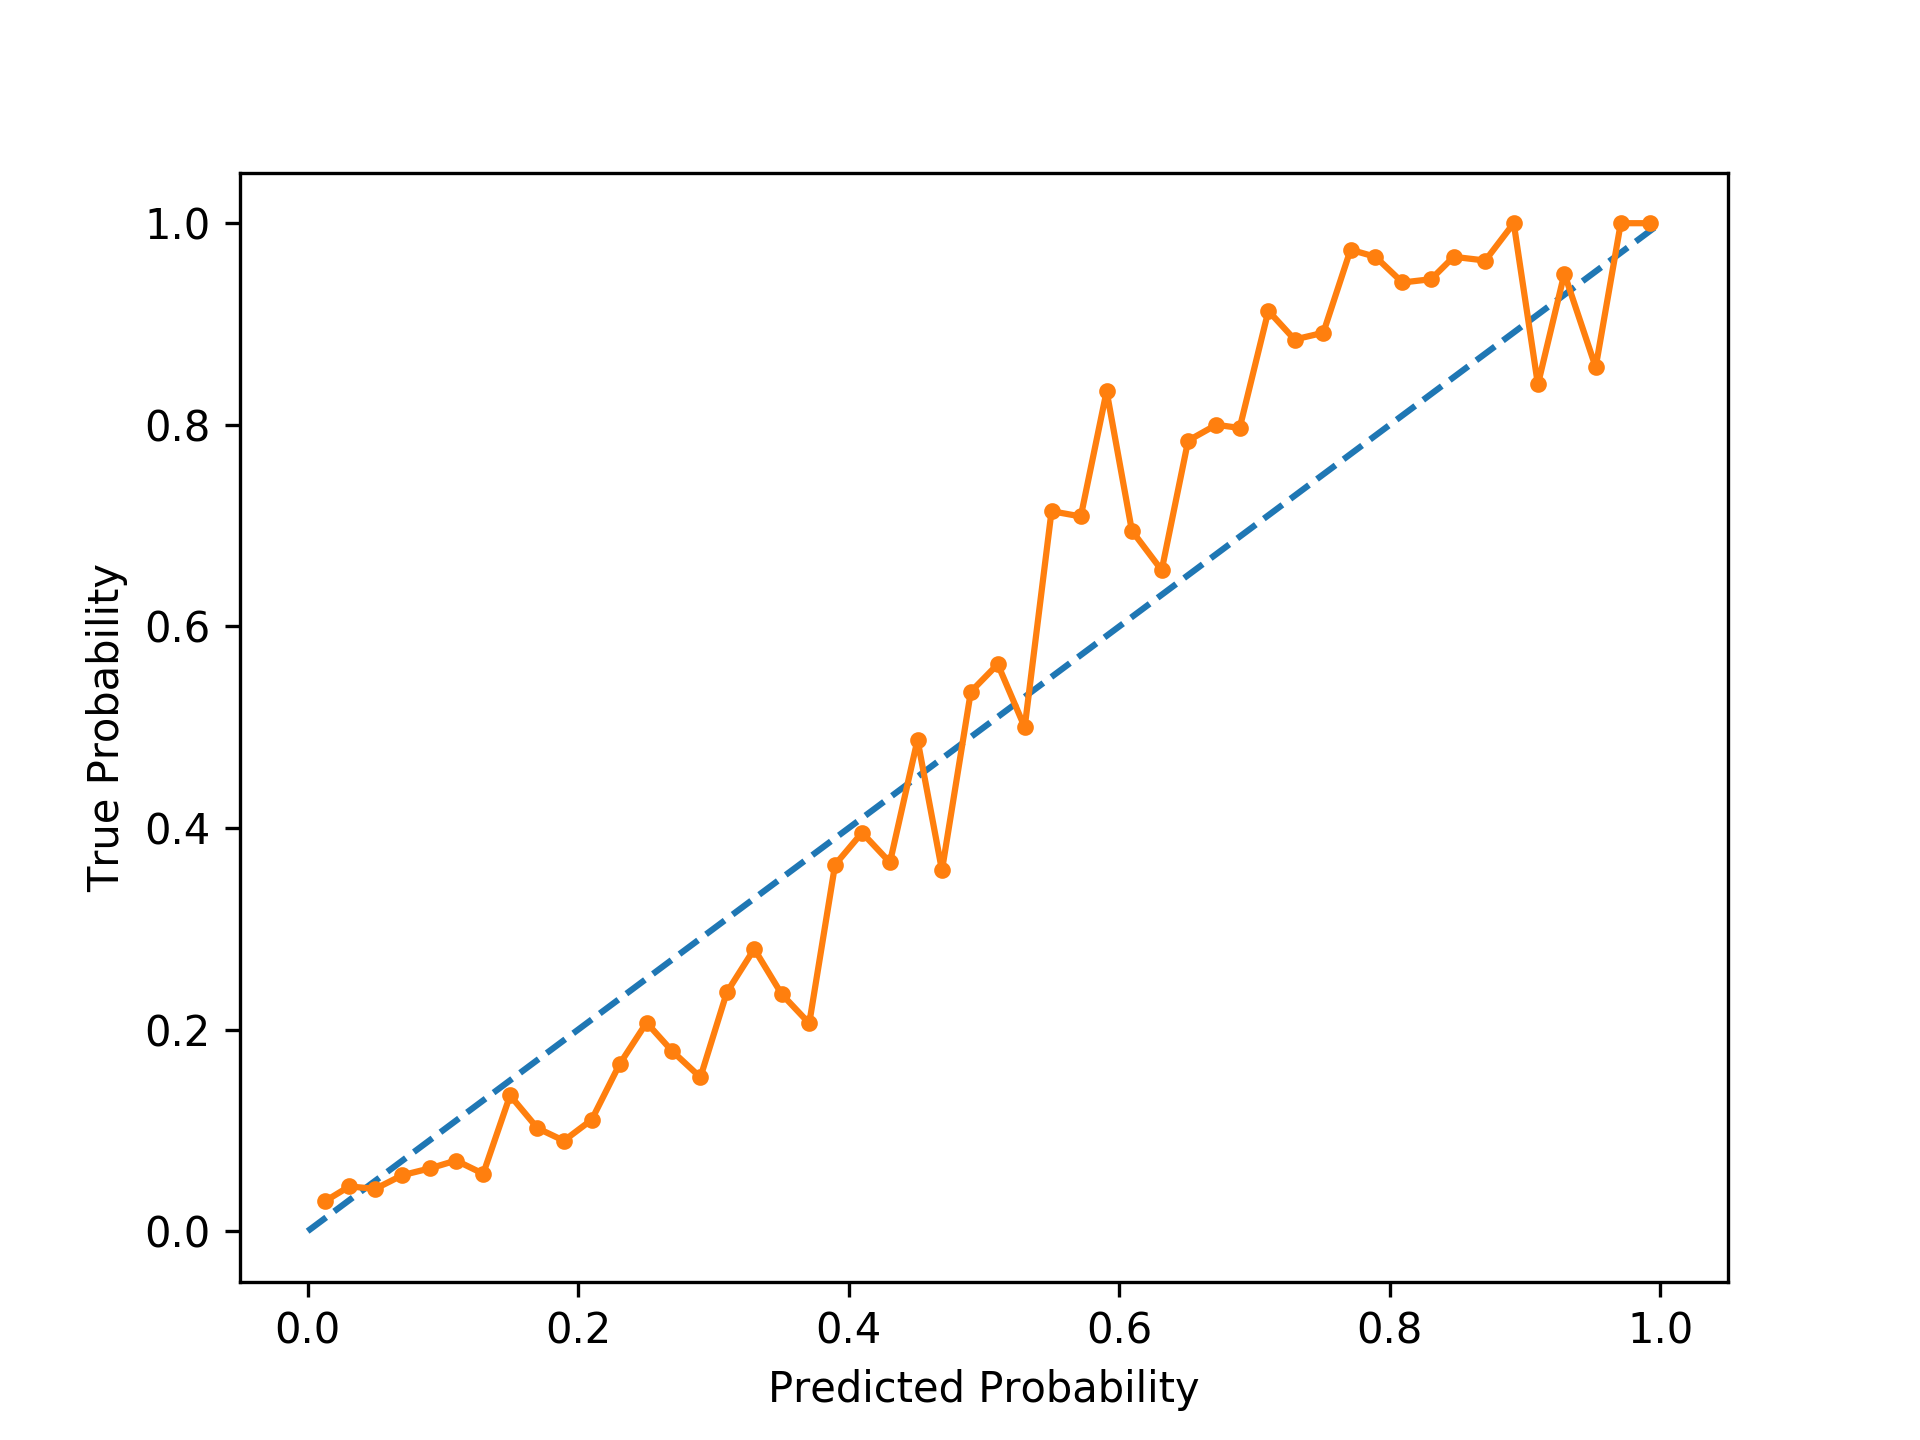
\includegraphics[width=0.7\linewidth]{figures/calibration_curve_raw_model.png}
 		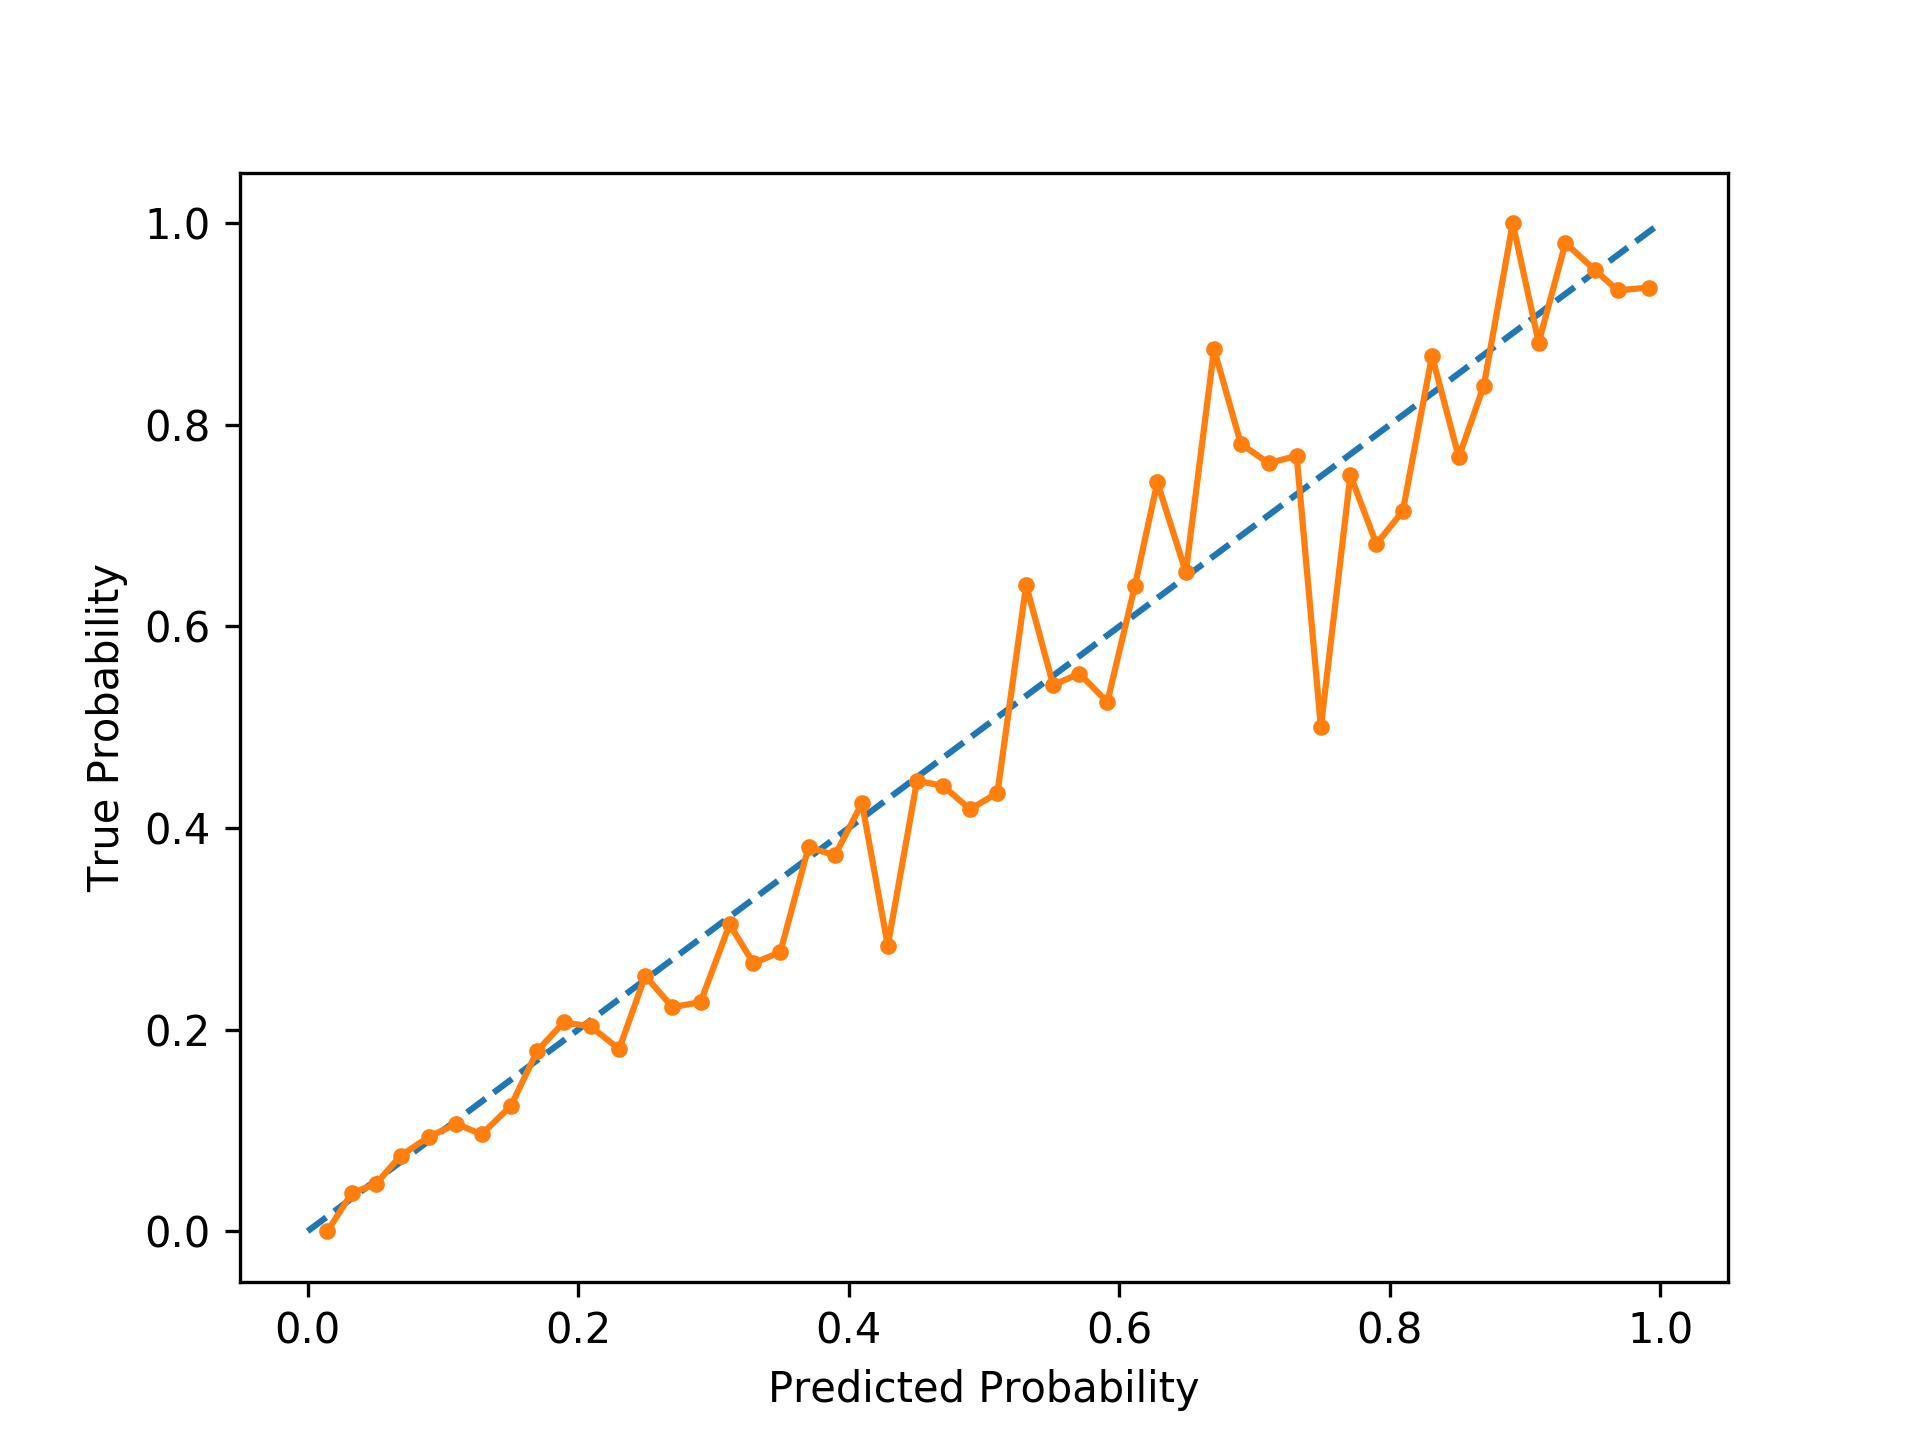
\includegraphics[width=0.7\linewidth]{figures/calibration_curve_calibrated_model.png}
 		\caption{Calibration Curve of Raw Model and Isotonic Calibrated Model}
 	\end{figure}
 	\subsection{Summary on Model Performances}
 	\paragraph{} Cross validations and the cross entropy (i.e. the log loss) were used to compare the relative performance across different types of models. It turned out that the uncalibrated random forest performed best.
 	
 	\begin{table}[H]
 		\centering
 		\begin{tabular}{l|c|c}
 			Model & Uncalibrated & Calibrated \\
 			\hline 
 			Logistic Regression & $0.5041 \pm 0.007183$ & $0.5301 \pm 0.01452$\\
 			Random Forest & \red{$0.3689 \pm 0.008212$} & $0.3919 \pm 0.009972$\\
 			Gradient Boosting & $0.4354 \pm 0.01348$ & $0.4277 \pm 0.002407$\\
 			Support Vector Classifier & $0.4523 \pm 0.01080$ & $0.4686 \pm 0.007865$ \\
%  			Deep Neural Network & & --
 		\end{tabular}
 		\caption{Relative Performances of Selected Models}
 	\end{table}
 	
 	Random forest also provided insights on relative importances of each features. From the feature importance plot, one can see that whether an assessment was taken in china or not, the visit day when the assessment was made, and the total PANSS score played were three major most correlated with the validity of assessment.
 	\begin{figure}[H]
 		\centering
 		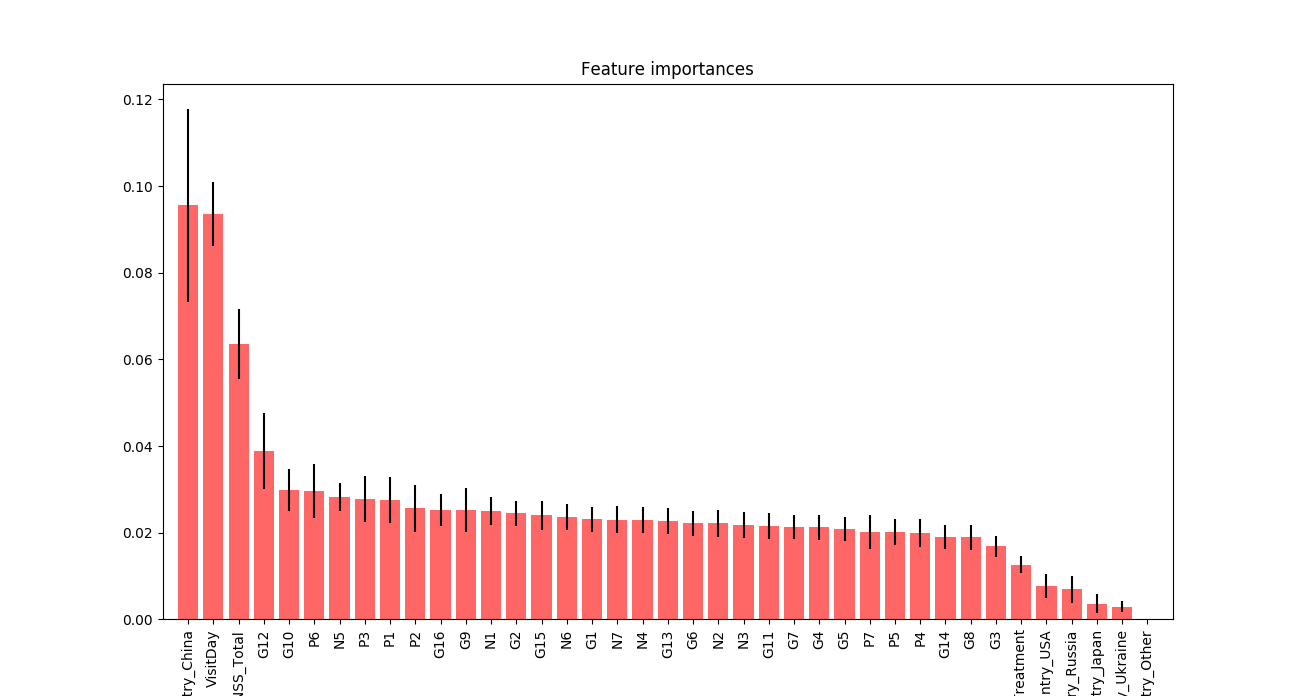
\includegraphics[width=0.9\linewidth]{figures/classification_feature_importance.png}
 		\caption{Feature Importance from Random Forest}
 	\end{figure}
 	
	\section{Appendix}
	\begin{figure}[H]
		\centering
		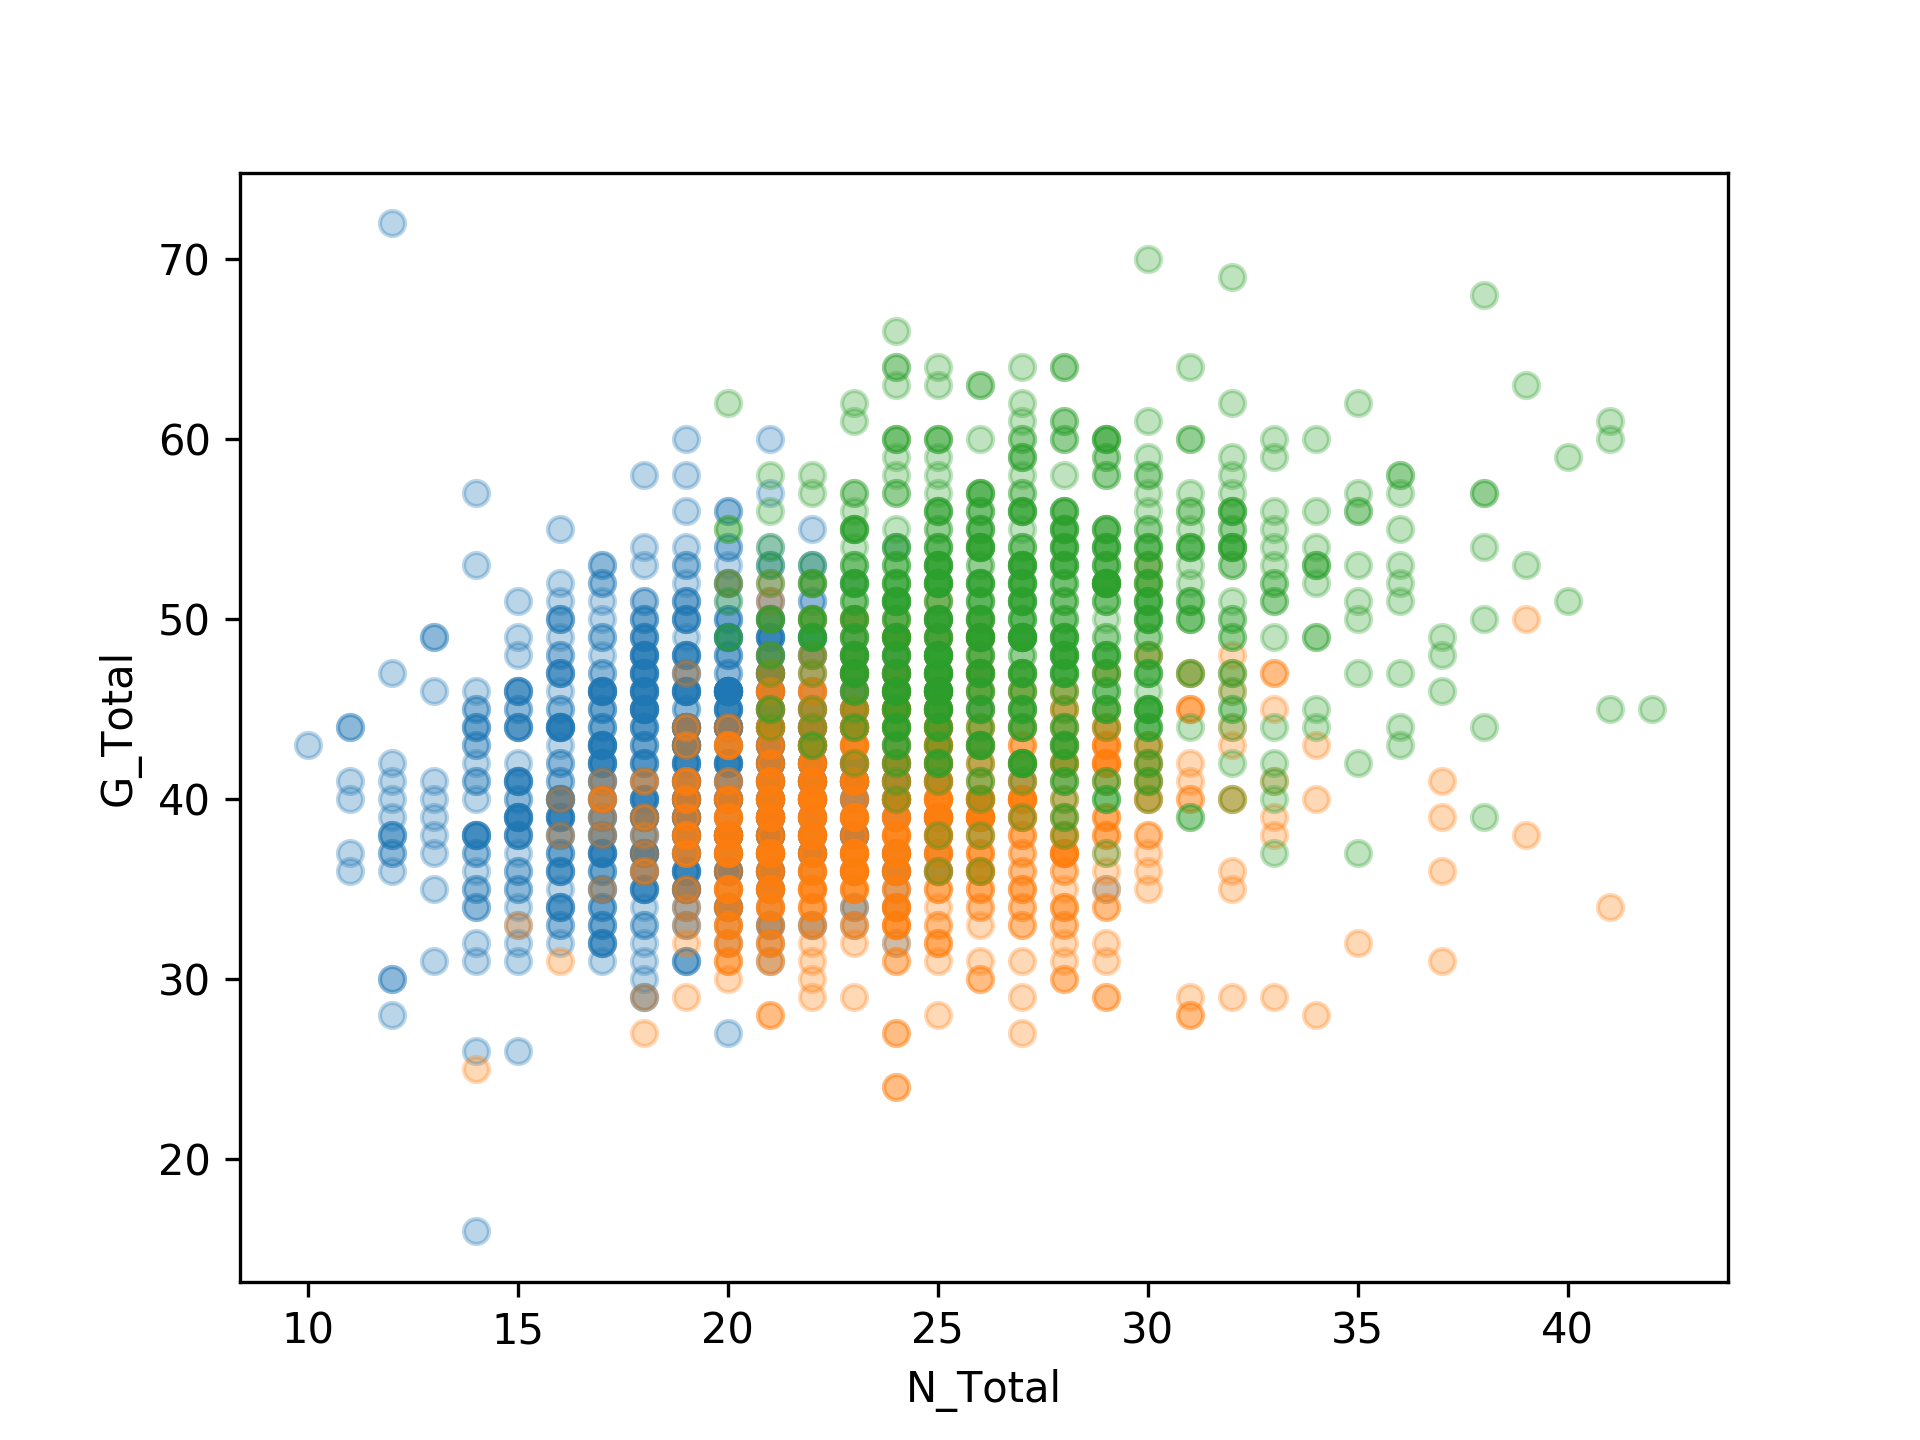
\includegraphics[width=0.7\linewidth]{figures/3_means_N_Total_G_Total.png}
		\caption{2D Plots of K-Mean Result}
	\end{figure}
	\begin{figure}[H]
	\centering
		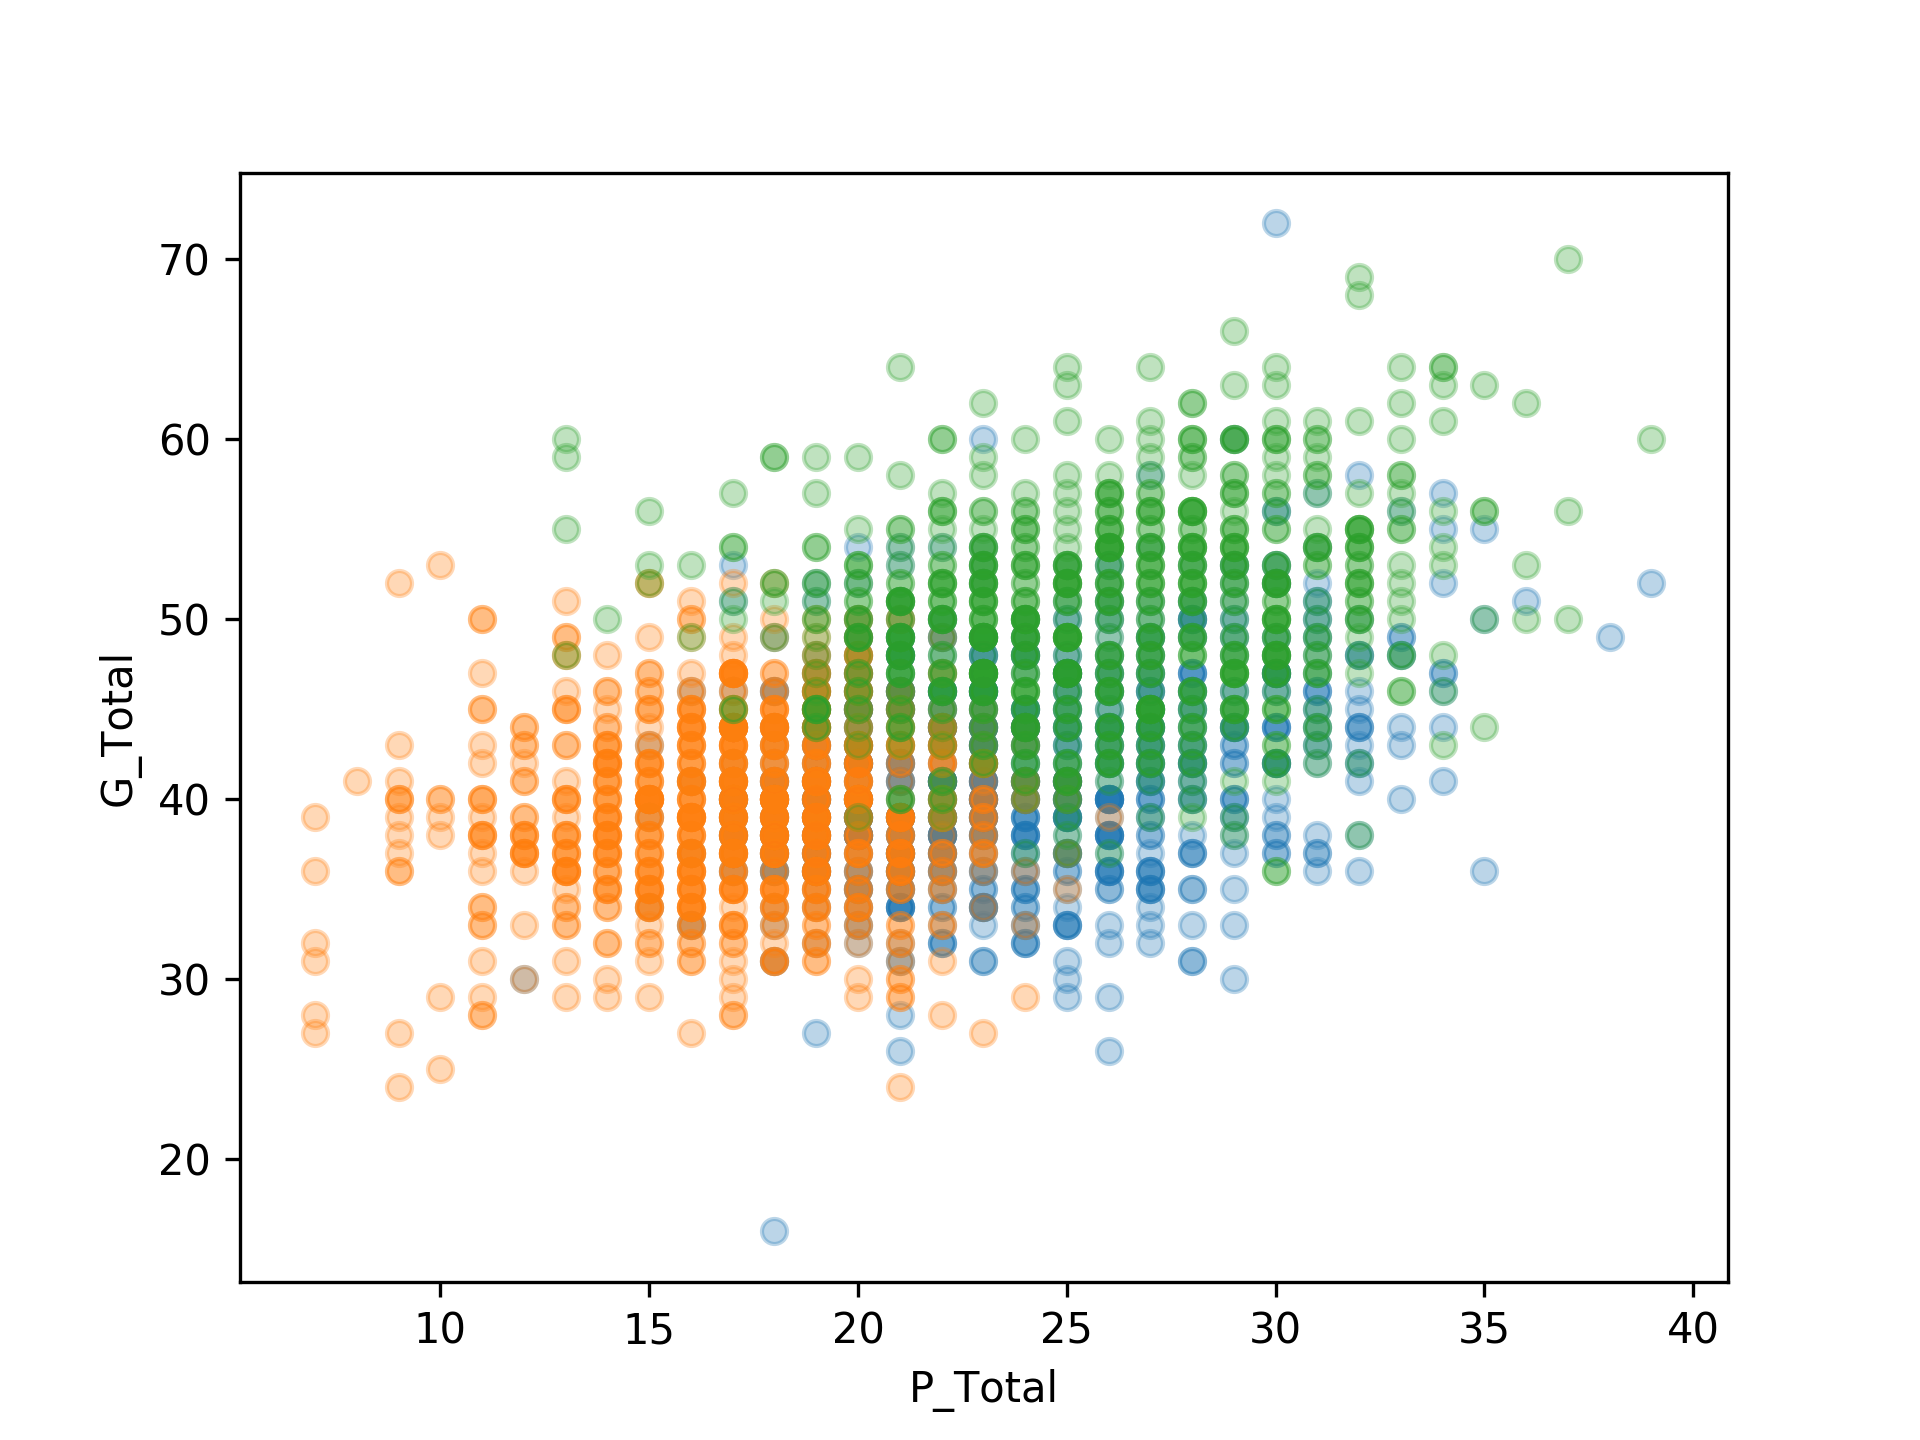
\includegraphics[width=0.7\linewidth]{figures/3_means_P_Total_G_Total.png}
		\caption{2D Plots of K-Mean Result}
	\end{figure}
	\begin{figure}[H]
		\centering
		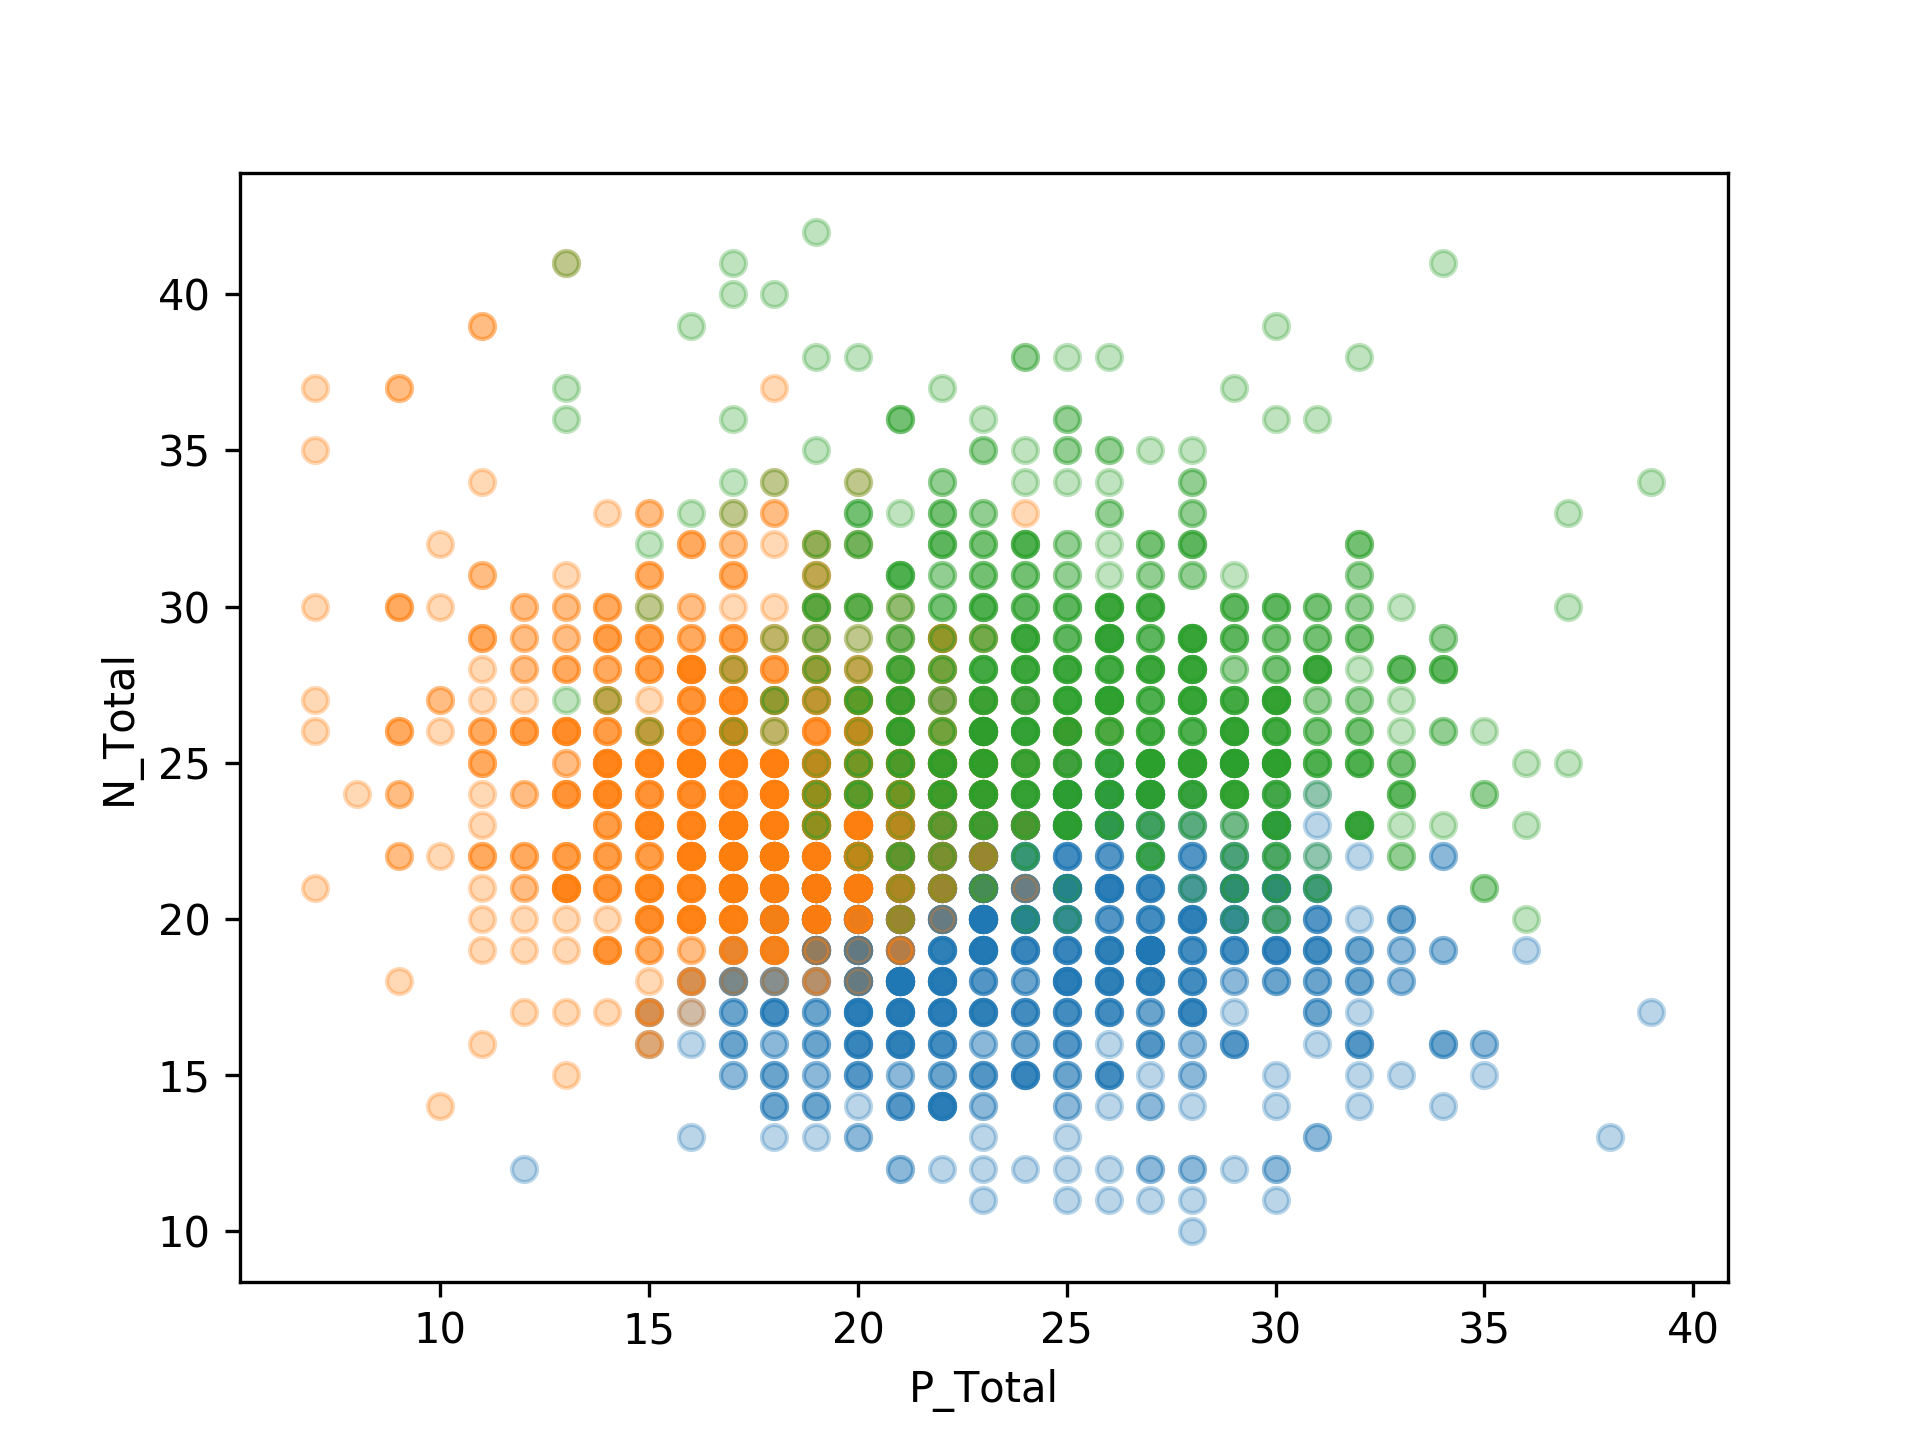
\includegraphics[width=0.7\linewidth]{figures/3_means_P_Total_N_Total.png}
		\caption{2D Plots of K-Mean Result}
	\end{figure}
\end{document}










